\chapter{Corrections and Systematic Uncertainties} \label{ch:error}

The large amount of data collected for the 8 TeV data set offers a unique chance to explore jet cross-sections using high statistics.   The double differential jet cross-section $d^{2}\sigma/dp_{T} \, d\eta$ is corrected using the Equation

\begin{equation}
	\frac{d^{2} \sigma^{jet}}{d\eta \, dp_{T}} = \frac{1}{\epsilon_{reco}} \frac{A_{trigger}}{\epsilon_{trigger}(p_{T})} \times C_{MC} (p_{T}) \times \frac{1}{A} \times \frac{1}{\mathscr{L}_{int}} \times \frac{dN^{2}_{jet}}{dp_{T} \, d\eta}
\label{eq:xsecdef}
\end{equation}

\noindent
where,

\begin{itemize}
  \item $\epsilon_{reco}$ is the efficiency for reconstructing the jet in the ALICE detector.
  \item $A_{trigger}$ is the acceptance for EMCal triggered events and $\epsilon_{trigger}(p_{T})$ is the EMCal trigger efficiency.  The factors correct for limitations in the EMCal and the overall factors are equal to one in Min Bias events.
  \item $C_{MC} (p_{T})$ is a correction factor due to detector effects and it allows for comparisons between the ALICE experiment and other experiments or theoretical calculations.  Bin-by-bin corrections are used to determine the factors.
  \item $\mathscr{L}_{int}$ is the integrated luminosity during the period when the data were recorded.
  \item $A$ is the geometrical detector acceptance.
  \item $\frac{dN^{2}_{jet}}{dp_{T} \, d\eta}$ is the uncorrected inclusive jet momentum spectrum.
  
\end{itemize}

By incorporating the additional terms in Equation \ref{eq:xsecdef} we can obtain a fully corrected inclusive jet cross-section that can be compared to theoretical calculations and other experiments.  Further cuts for the geometric acceptance, corrections for detector effects, and efficiency calculations need to be accounted for to measure fully corrected jets.  This chapter will conclude with a presentation of the systematic uncertainties that are reported with the final jet cross-sections

\section{Uncorrected Jet Spectra}

This analysis measured inclusive jet cross-sections for radii between 0.2 and 0.4.  Figures \ref{fig:uncorrectedjetR02}, \ref{fig:uncorrectedjetR03}, and \ref{fig:uncorrectedjetR04} show the uncorrected $p_{T}$ spectra for inclusive jets from both Min Bias and EMCal triggered data.  It is evident from these figures that the EMCal triggered data greatly extend the kinematic reach of the measured jet spectra, to about 200 GeV/c.  The EMCal triggered data introduce a bias at low-$p_{T}$ as seen in the different distribution shapes. 

\afterpage{%
\begin{figure}
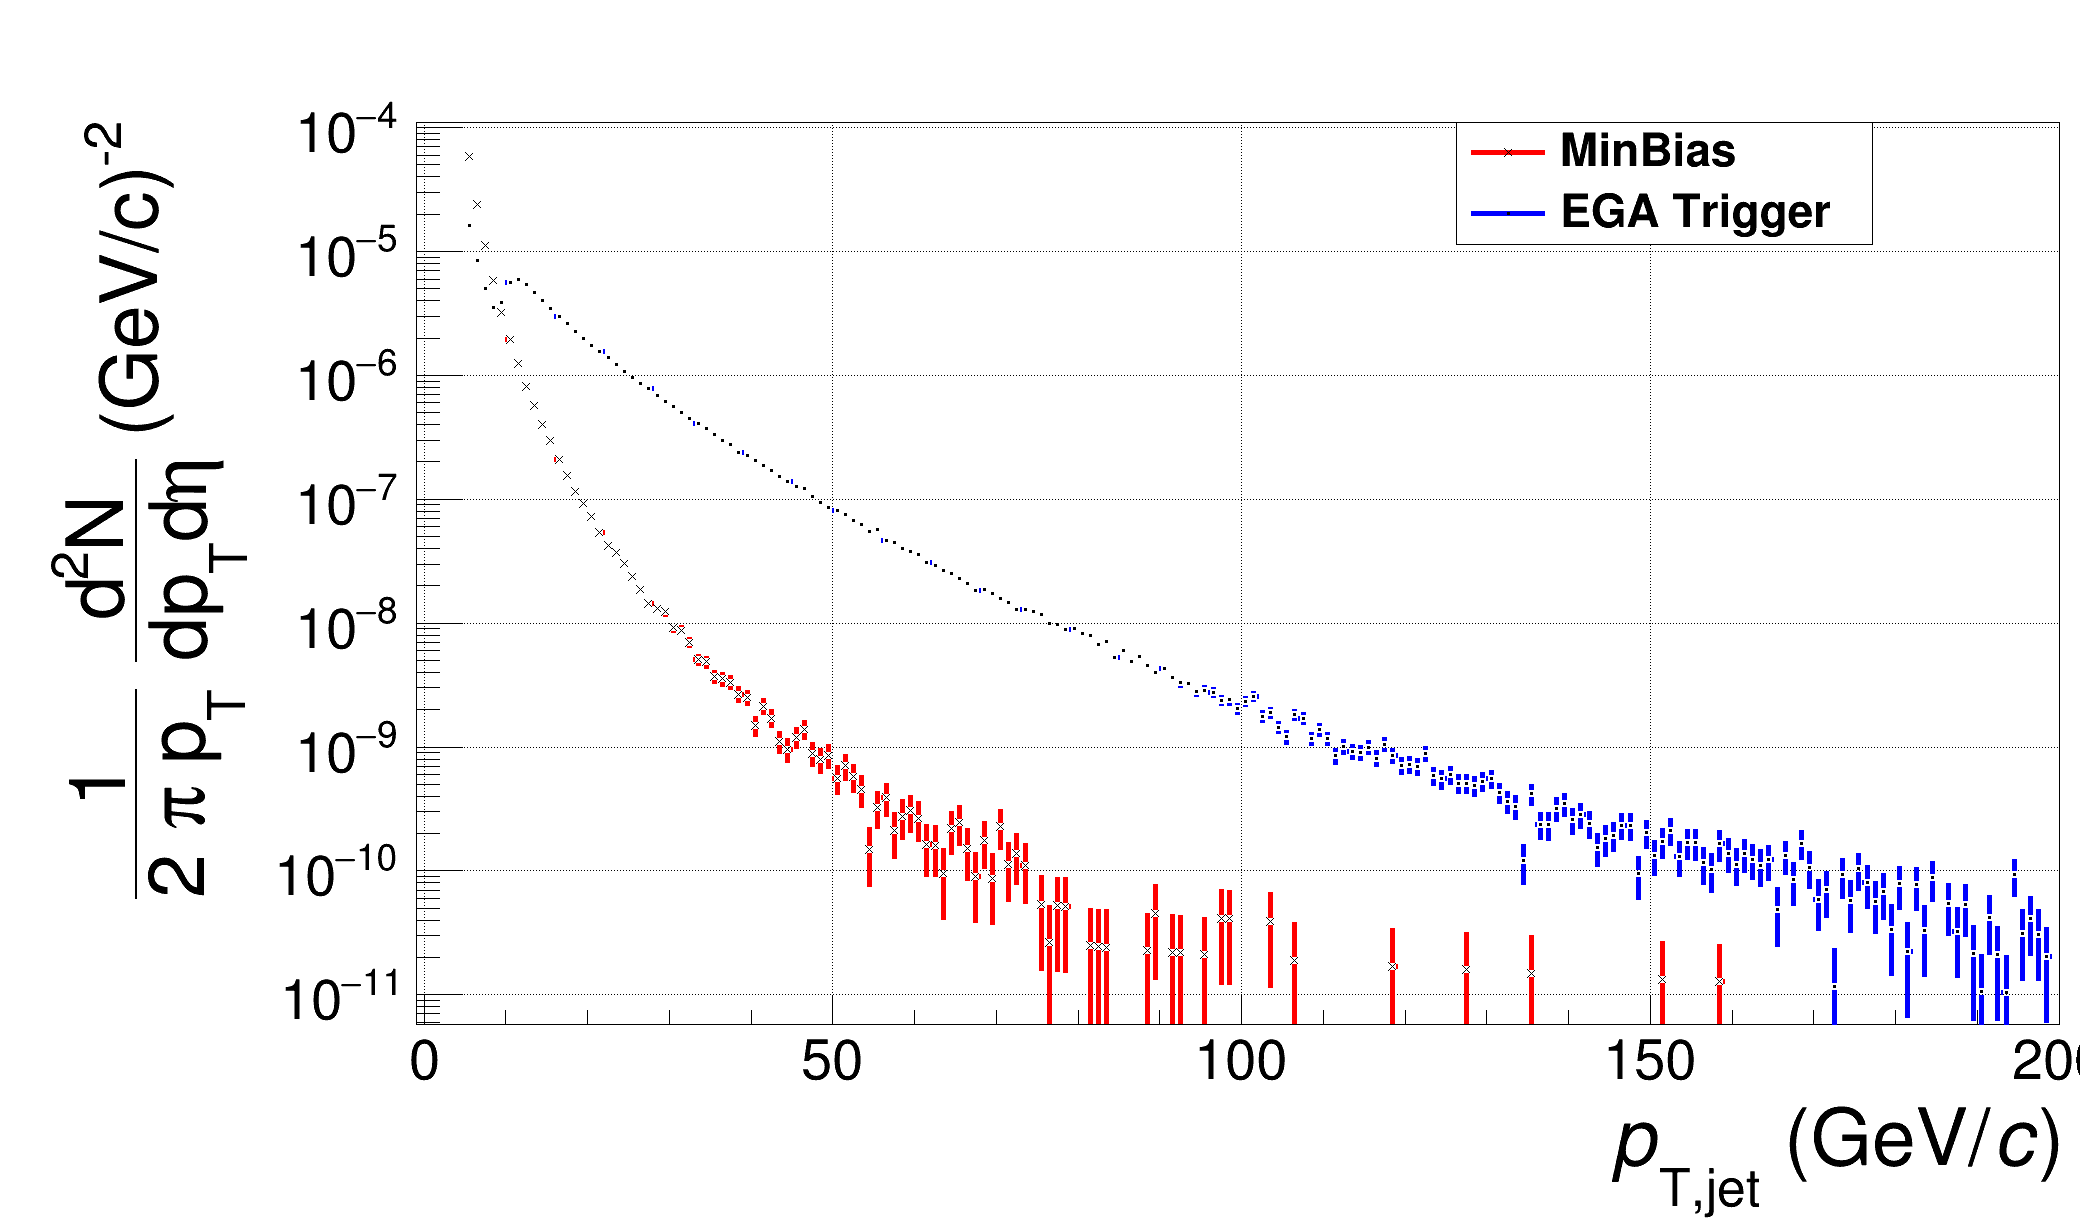
\includegraphics[width=\linewidth]{IPYNB_Systematics_R02MBandEGARAW}
\centering
\caption{Uncorrected inclusive R = 0.2 jet spectra from the 8 TeV Min Bias and EMCal triggered data}
\label{fig:uncorrectedjetR02}
\end{figure}

\begin{figure}
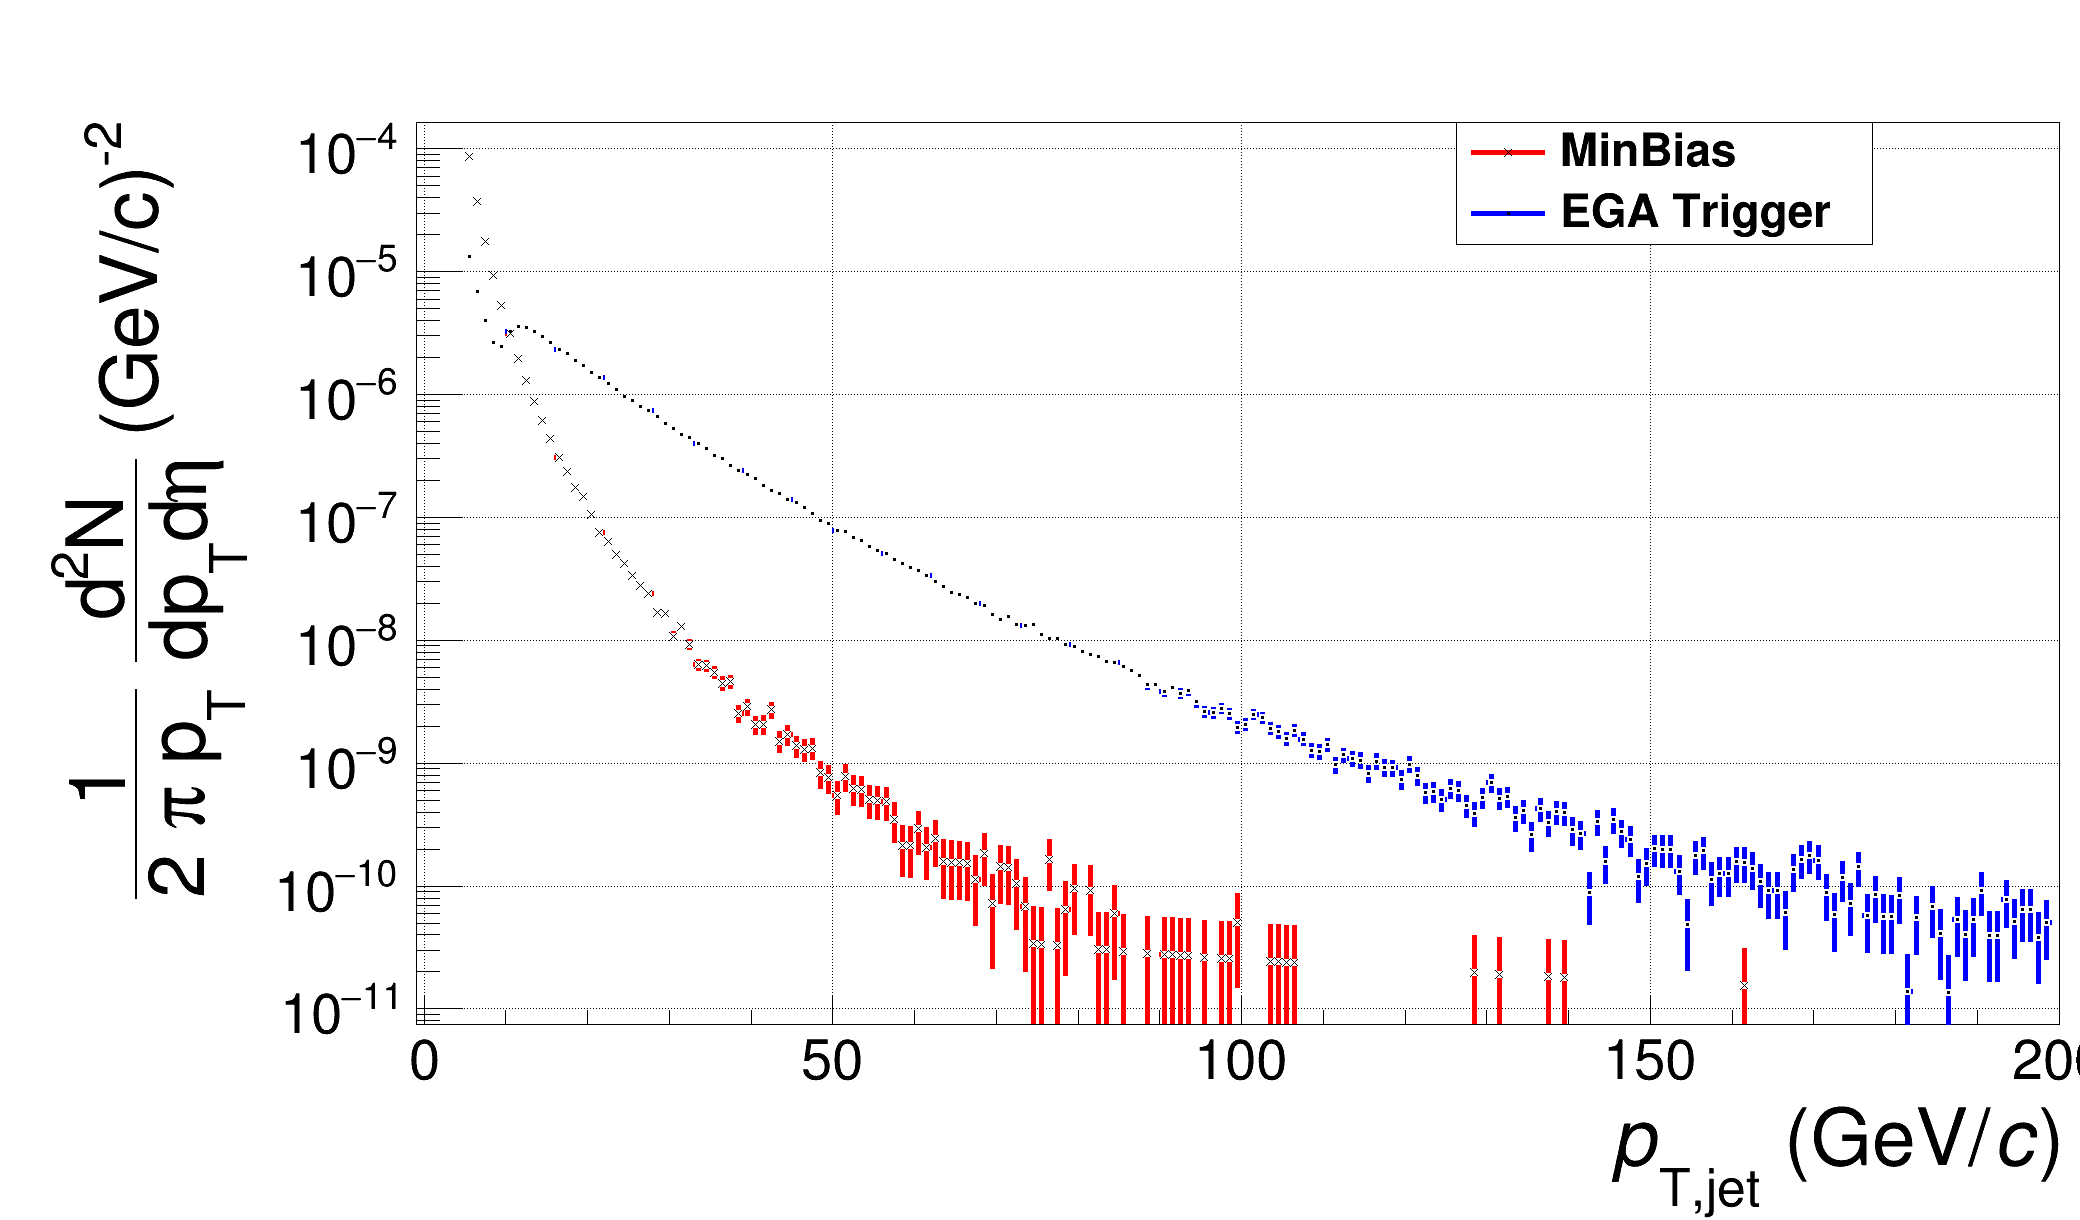
\includegraphics[width=\linewidth]{IPYNB_Systematics_R03MBandEGARAW}
\centering
\caption{Uncorrected inclusive R = 0.3 jet spectra from the 8 TeV Min Bias and EMCal triggered data}
\label{fig:uncorrectedjetR03}
\end{figure}

\begin{figure}
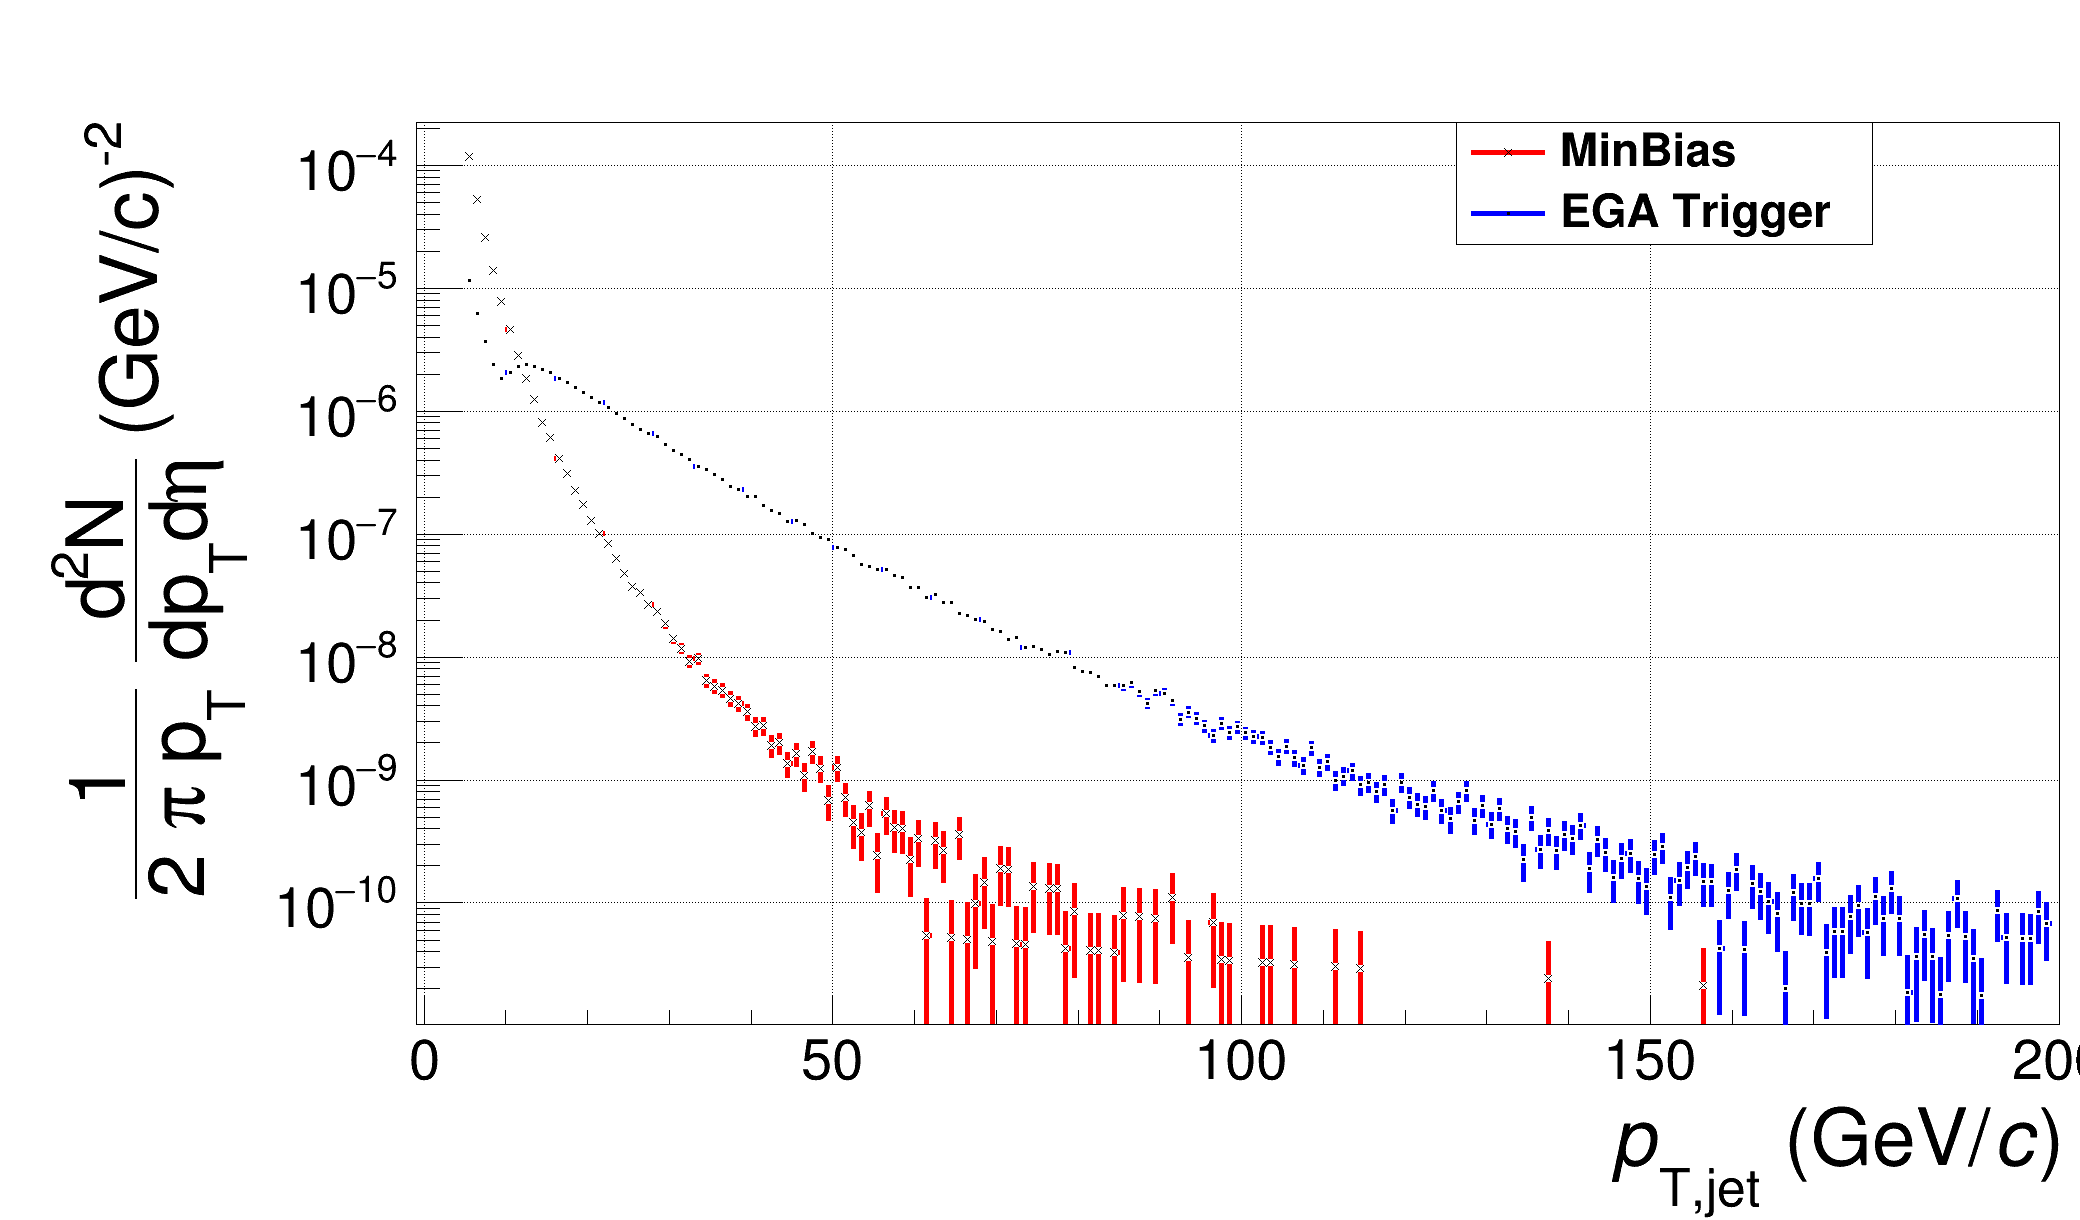
\includegraphics[width=\linewidth]{IPYNB_Systematics_R04MBandEGARAW}
\centering
\caption{Uncorrected inclusive R = 0.4 jet spectra from the 8 TeV Min Bias and EMCal triggered data}
\label{fig:uncorrectedjetR04}
\end{figure}

\clearpage
}


\section{Acceptance Correction}
Jet cross-sections and ratios of cross-sections are reported over the full azimuthal angle and pseudorapidity acceptance in this thesis.  Because jets are constrained to the EMCal, a geometric factor was used to correct for the limited acceptance of the detector.  This thesis explored jet radii between 0.2 and 0.4 in order to study the effects of wide angle radiation on jet fragmentation.  Due to these geometric corrections the centroid of a jet is constrained to,

\begin{equation}
|\eta_{jet}| \leq 0.7 - R, \; 1.4 + R \leq \phi_{jet} \leq 3.14 -R.
\label{eq:jetconstration}
\end{equation}

\begin{equation}
A(p_{T}) = \frac{(1.4 - 2R) \times (1.745 - 2R)}{2 \pi}.
\label{eq:acceptance}
\end{equation}

For jets between R = 0.1 through R = 0.5 the following jet acceptance corrections are given in Table 5.2.

\begin{table}[hb]
\label{tab:AcceptanceFactor}
\begin{center}
\caption{EMCal jet acceptance for radii 0.1 - 0.5.}
\begin{tabular}[b]{|c|c|c|}
	\hline
	Jet R & $ A $ \\ \hline
	0.1 & 0.296 \\ \hline
	0.2 & 0.214\\ \hline
	0.3 & 0.146\\ \hline
	0.4 & 0.091\\ \hline
	0.5 & 0.048\\ \hline
\end{tabular}
\end{center}

\end{table}

\section{EMCal Triggered Data}

As discussed in Chapter \ref{ch:alice}, the ALICE detector is unable to record all events that occur in the experiment.   The use of a trigger allows for events with rare processes to be saved with a high efficiency and analyzed.  The EMCal trigger used for the 8 TeV data extends the kinematic reach of the spectra and the sample of jets from the data.  This thesis looked at the two primary Level-1 triggers configured for the EMCal, the jet trigger and the gamma trigger\cite{Bourrion:2010js}.  Although both of the Level-1 triggers were investigated in this analysis, only the gamma trigger was ultimately used for the final jet cross-sections and spectra.  

The jet trigger is a patch consisting of 32 x 32 EMCal towers, roughly the same size as a R = 0.3 jet.  The patch samples all possible tower configurations to see if the patch meets the minimum predefined energy threshold.  Once this threshold is surpassed the event is recorded and tagged as a jet triggered event.  A similar procedure is followed for the gamma trigger, but with a smaller patch region of 4 x 4 towers and a different energy threshold.  

The bump at low-$p_{T}$ seen in the EMCal data points of Figures \ref{fig:uncorrectedjetR02}, \ref{fig:uncorrectedjetR03}, and \ref{fig:uncorrectedjetR04} is the trigger turn on curve. The peak of the triggered data corresponds to the trigger threshold for the EGA trigger.  A jet in the EMCal acceptance should fire the jet trigger and the gamma should fire due to the presence of a photon or electron. It is also possible for a jet to fire both triggers.  The EMCal triggered events have a higher yield of jets compared to the Min Bias spectra. The triggered data are downscaled.  This corrects the enhancement and makes the triggered data equivalent to the Min Bias data.  

The triggered data also need to be corrected by reconstructing the jet that fired the jet trigger.  This analysis was concerned with analyzing jets that fired the trigger and removing any bias to processes outside of jet production. Therefore jets were matched to the trigger patch.  In order to only correct jets that fired a trigger in the EMCal the following procedure was implemented.  First both the jet and gamma trigger patches were reconstructed offline.  Next the energy thresholds were set for each trigger.  Then the centroid of the trigger was found by finding the center-of-mass for each reconstructed patch in $\eta$ and $\phi$.  After all patches were reconstructed and their weighted centroids found, each patch was geometrically matched to the jet centroid.  The geometrical matching requirement followed a simple quadratic relationship which constrained the center of the trigger to inside the jet radius,

\begin{equation}
\sqrt{ ( \phi_{jet} - \phi_{EMCal patch} )^{2} + ( \eta_{jet} - \eta_{EMCal patch} )^{2}}  \leq R_{jet} .
\label{eq:triggermatch}
\end{equation}

\begin{figure}[h]
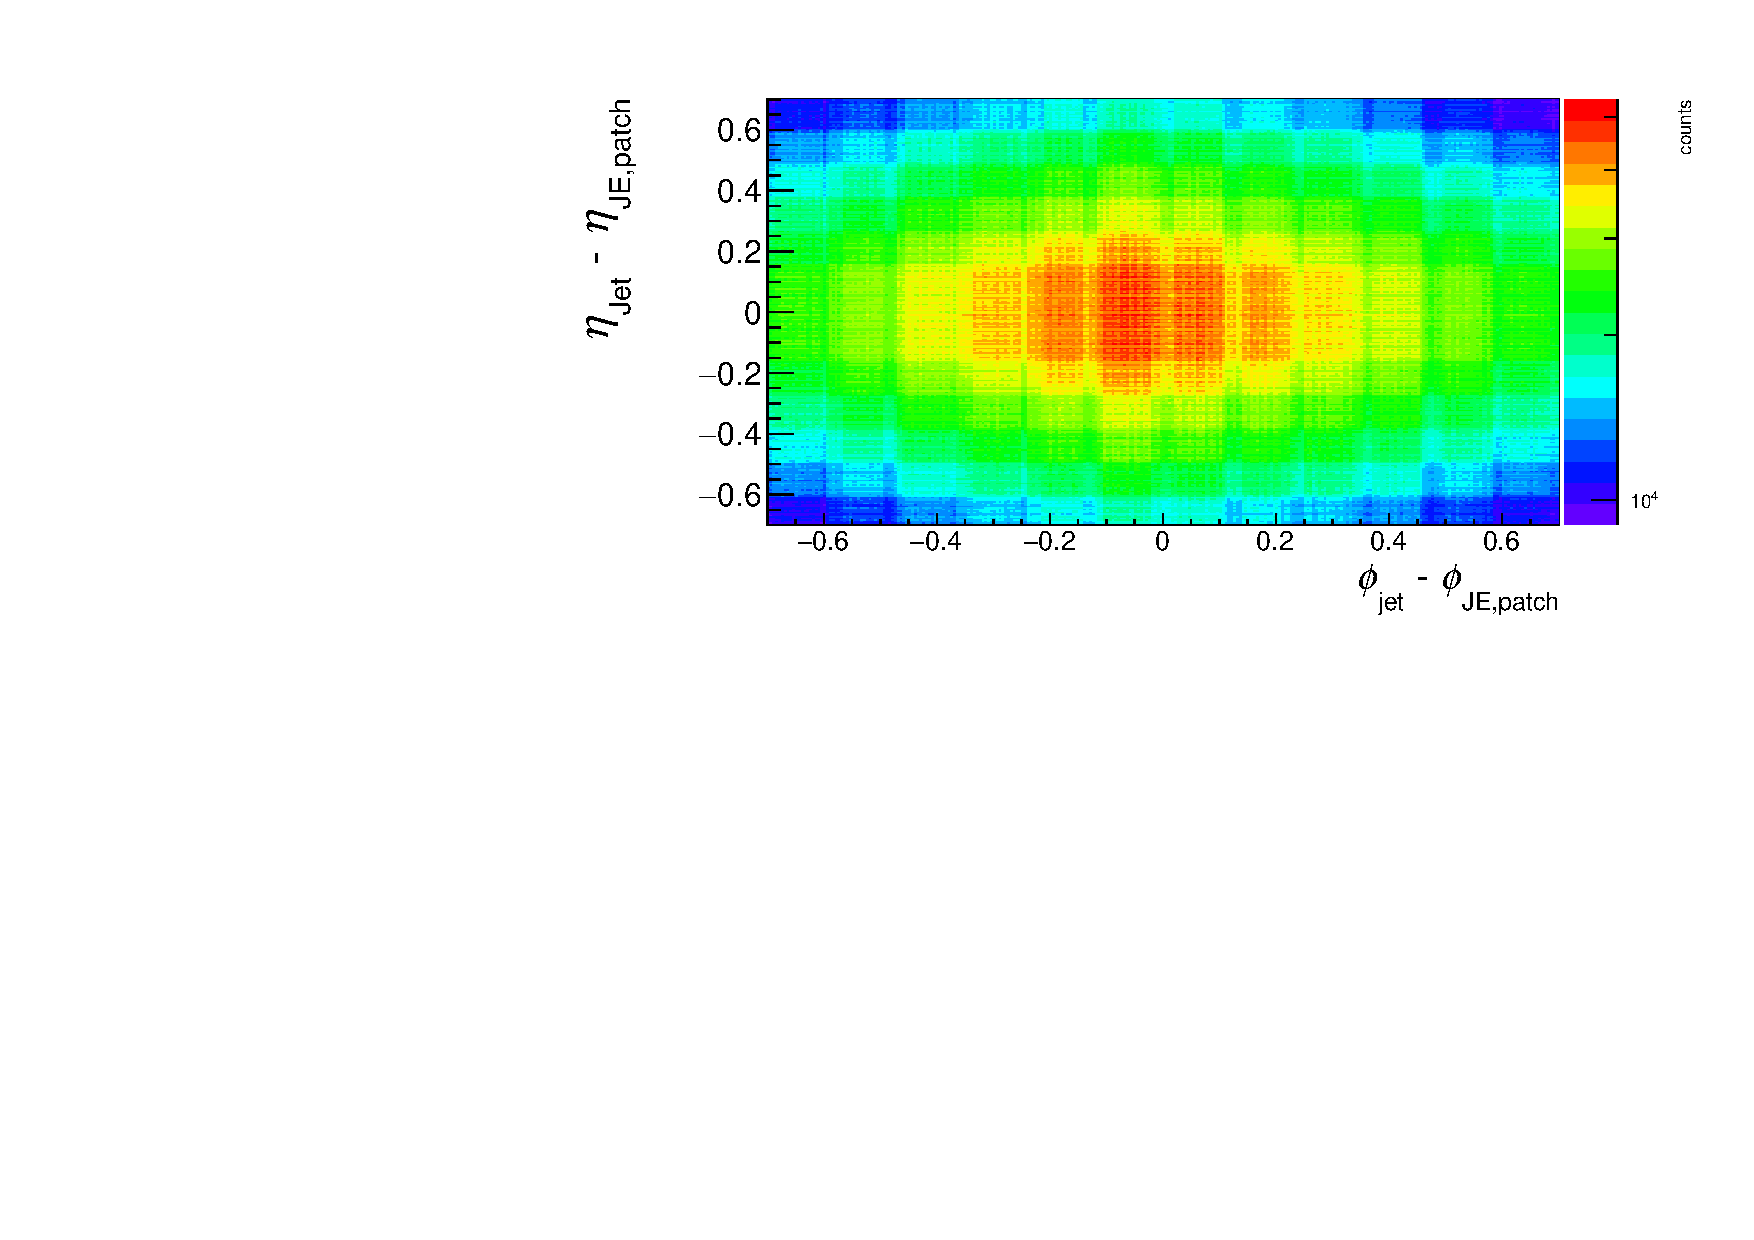
\includegraphics[width=\linewidth]{JEpatchetaphi}
\centering
\caption{Distance to closest reconstructed jet patch to R = 0.2 jet with the EMCal triggered data.}
\label{fig:DisJetEJE}
\end{figure}

\begin{figure}[h]
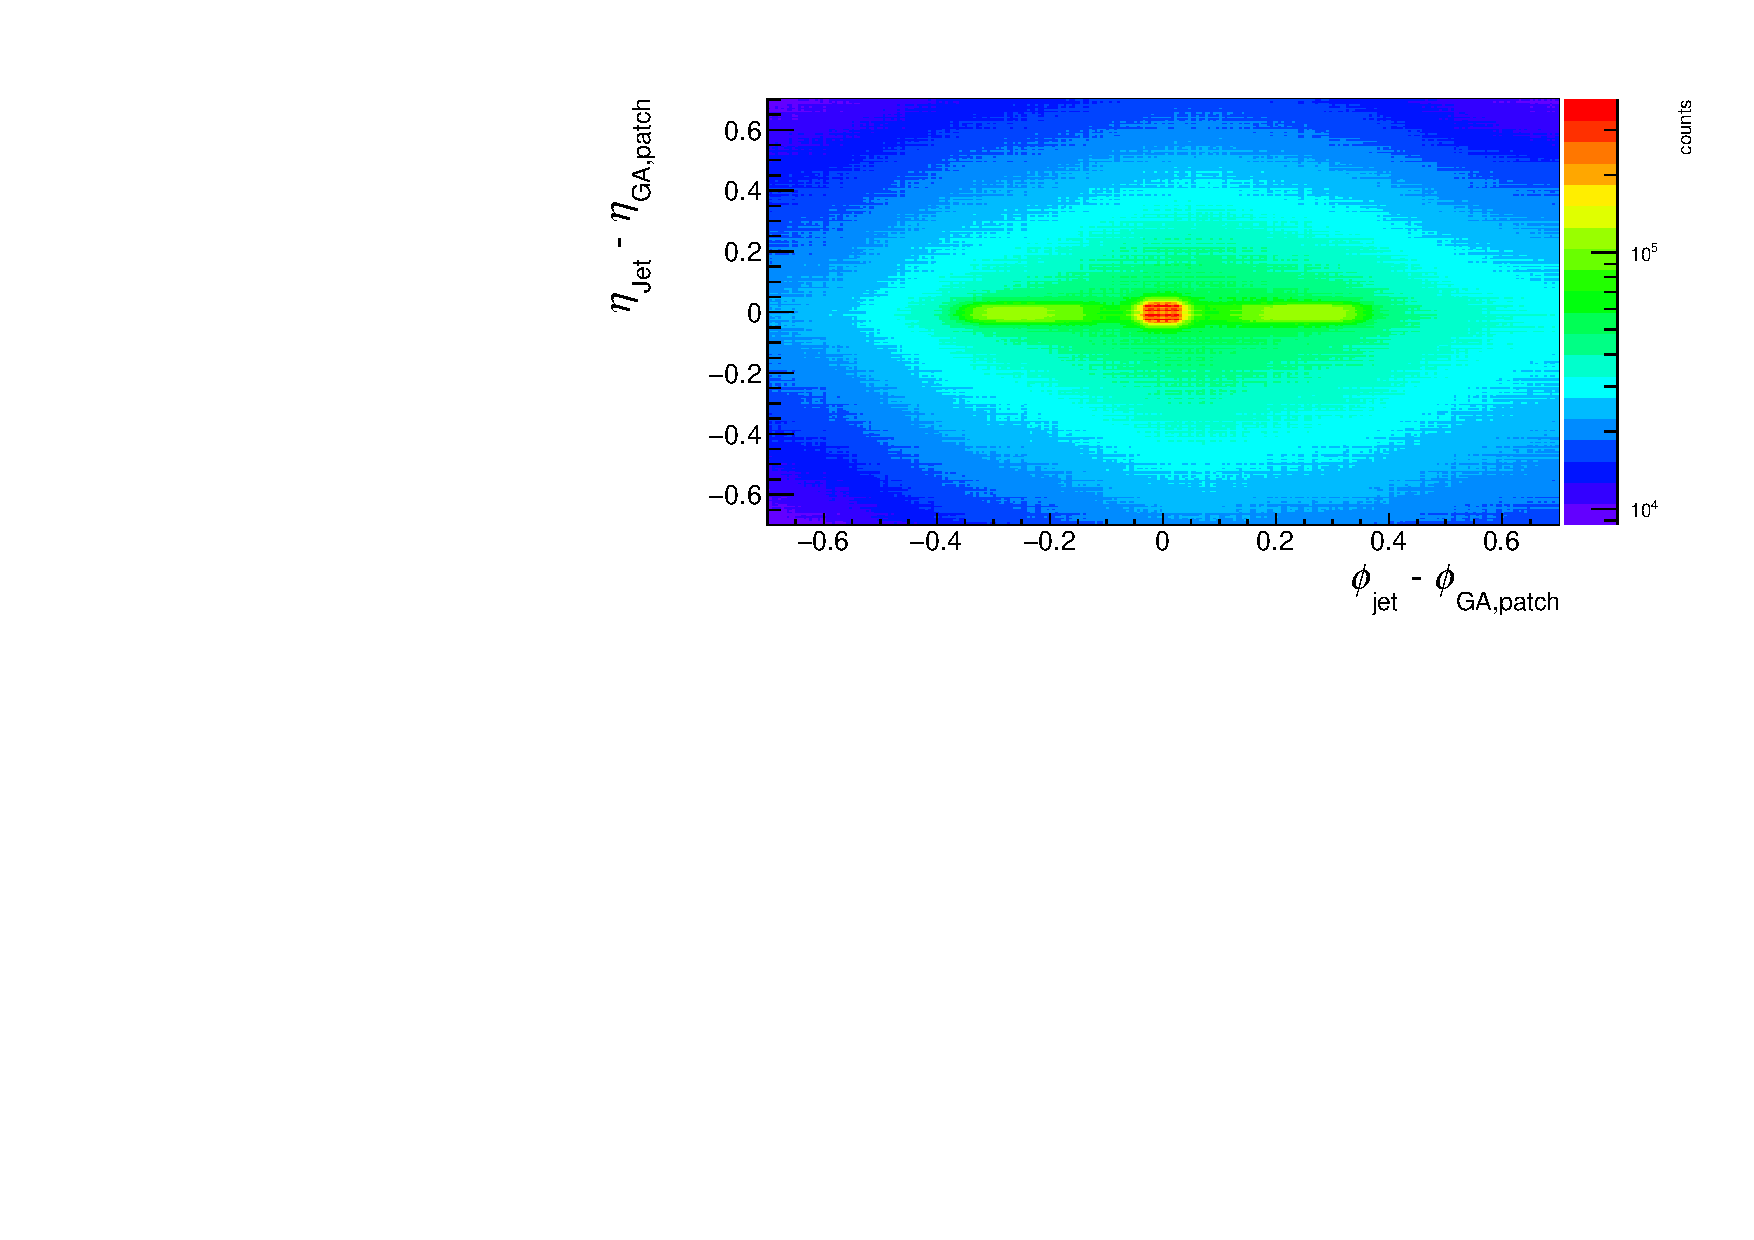
\includegraphics[width=\linewidth]{jetgammaetaphi}
\centering
\caption{Distance to closest reconstructed gamma patch to R = 0.2 jet with EMCal triggered data.}
\label{fig:DisJetEGA}
\end{figure}

\noindent
If a match between the gamma patch and a jet is made, the jet is flagged as triggering the event.  Figures \ref{fig:DisJetEJE} and \ref{fig:DisJetEGA} show the distance between a reconstructed jet and its closest reconstructed EMCal trigger patch for R = 0.2 jets using the triggered data.  Since a trigger patch may be fired if two or more jets are within the geometric area of the trigger patch this could lead to double counting.  In order to correct for this, the jet spectra from the triggered data is scaled by the number of triggers, $N_{trig}$, fired that fell within the jet.  

Once this correction was implemented, the triggered data were then downscaled in order to combine it with the Min Bias data.  The downscale factors, shown in Figure \ref{fig:EMCalDownScale}, were obtained by taking the ratio of the EMCal jet spectra to the Min Bias jet spectra and fitting the plateau region to a line.  The approximate scale factors are 6566 $\pm$ 326 for R = 0.2, 4383 $\pm$ 242 for R = 0.3, and 4287 $\pm$ 246 for R = 0.4.  Below $\sim$40 GeV/\textit{c}, the efficiency in the triggered data is changing rapidly and hard to determine.  The Min Bias data are sufficient for measuring the low momentum range of the jet spectrum.  The downscaled EMCal data are used at 40 GeV/\textit{c} and above.  The scale factors seen in Figure \ref{fig:EMCalDownScale} were obtained after the Bin-by-Bin corrections were applied to the data.


\begin{figure*}[t!]
$\begin{array}{rl}
    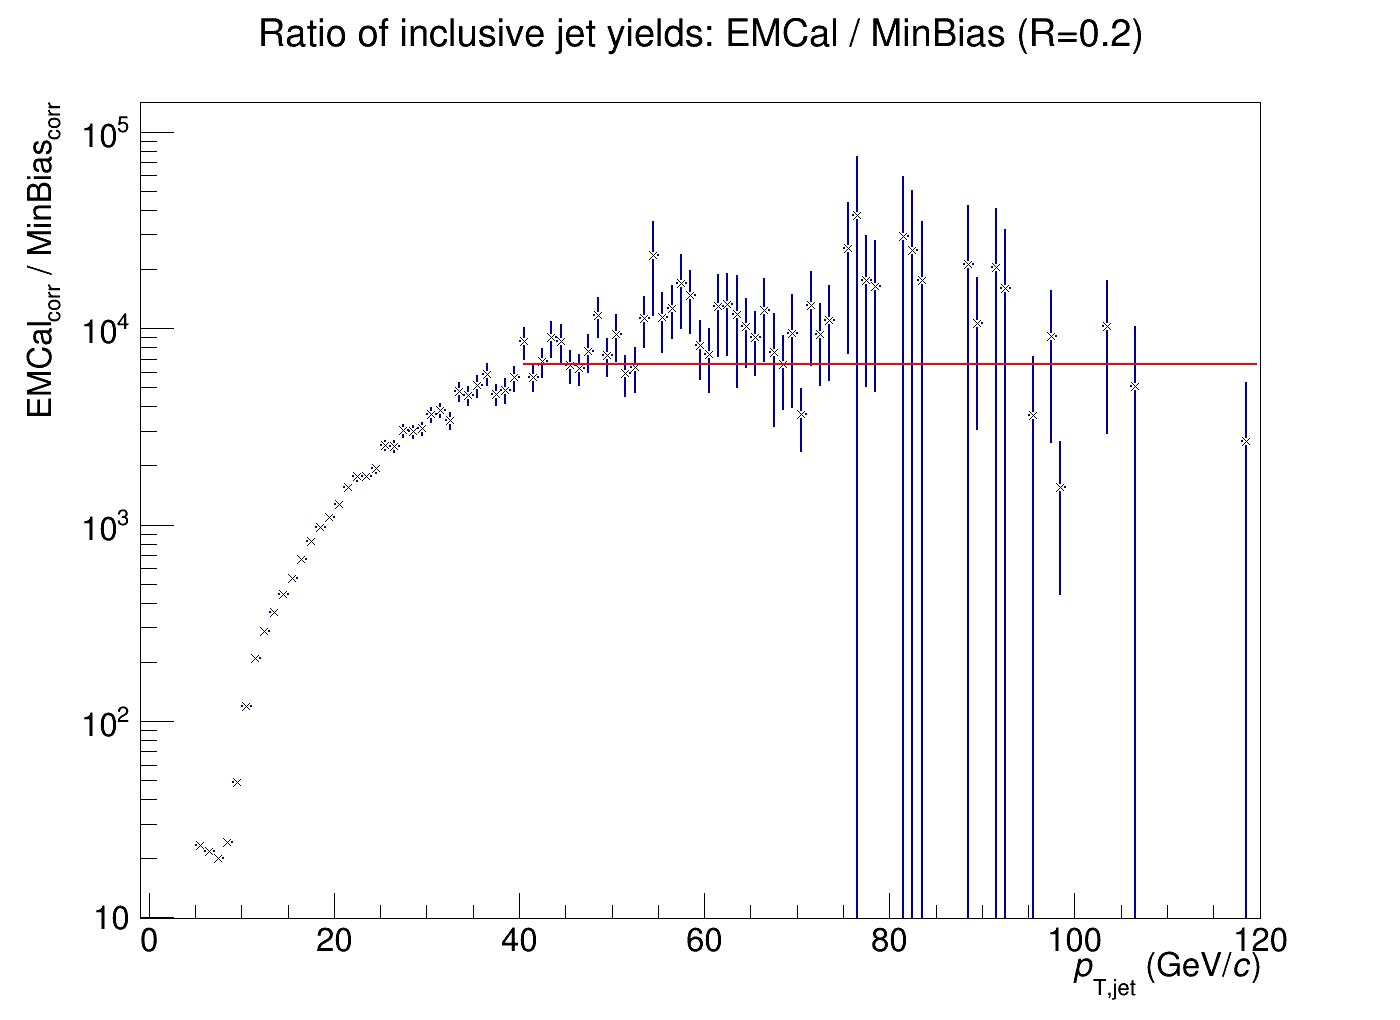
\includegraphics[width=0.5\textwidth]{R02TriggerYields} &
    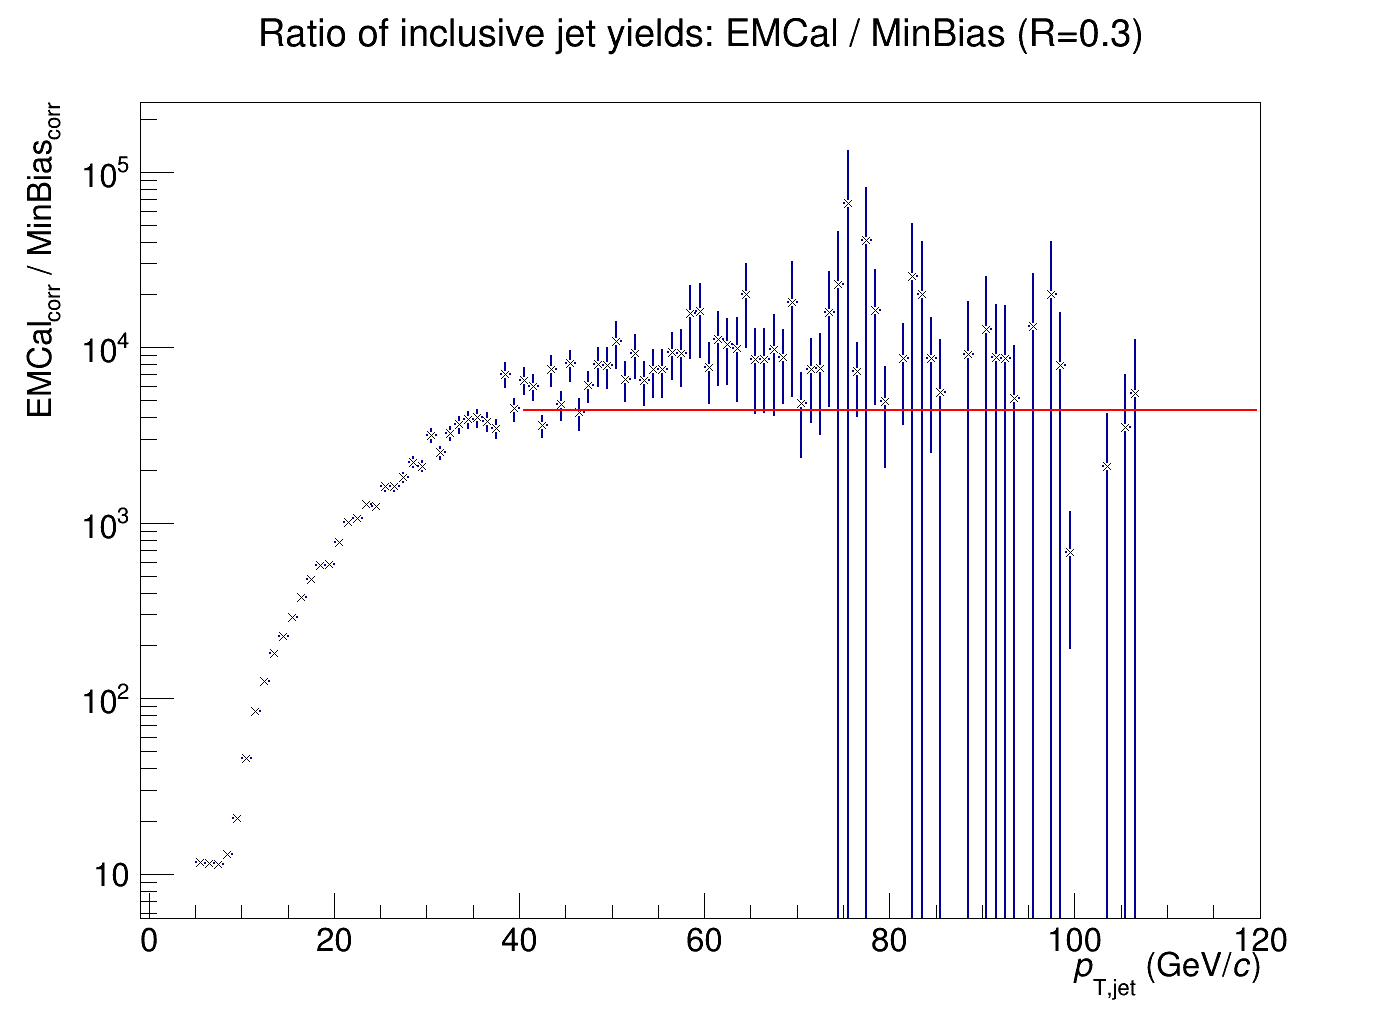
\includegraphics[width=0.5\textwidth]{R03TriggerYields}\\
    \multicolumn{2}{c}{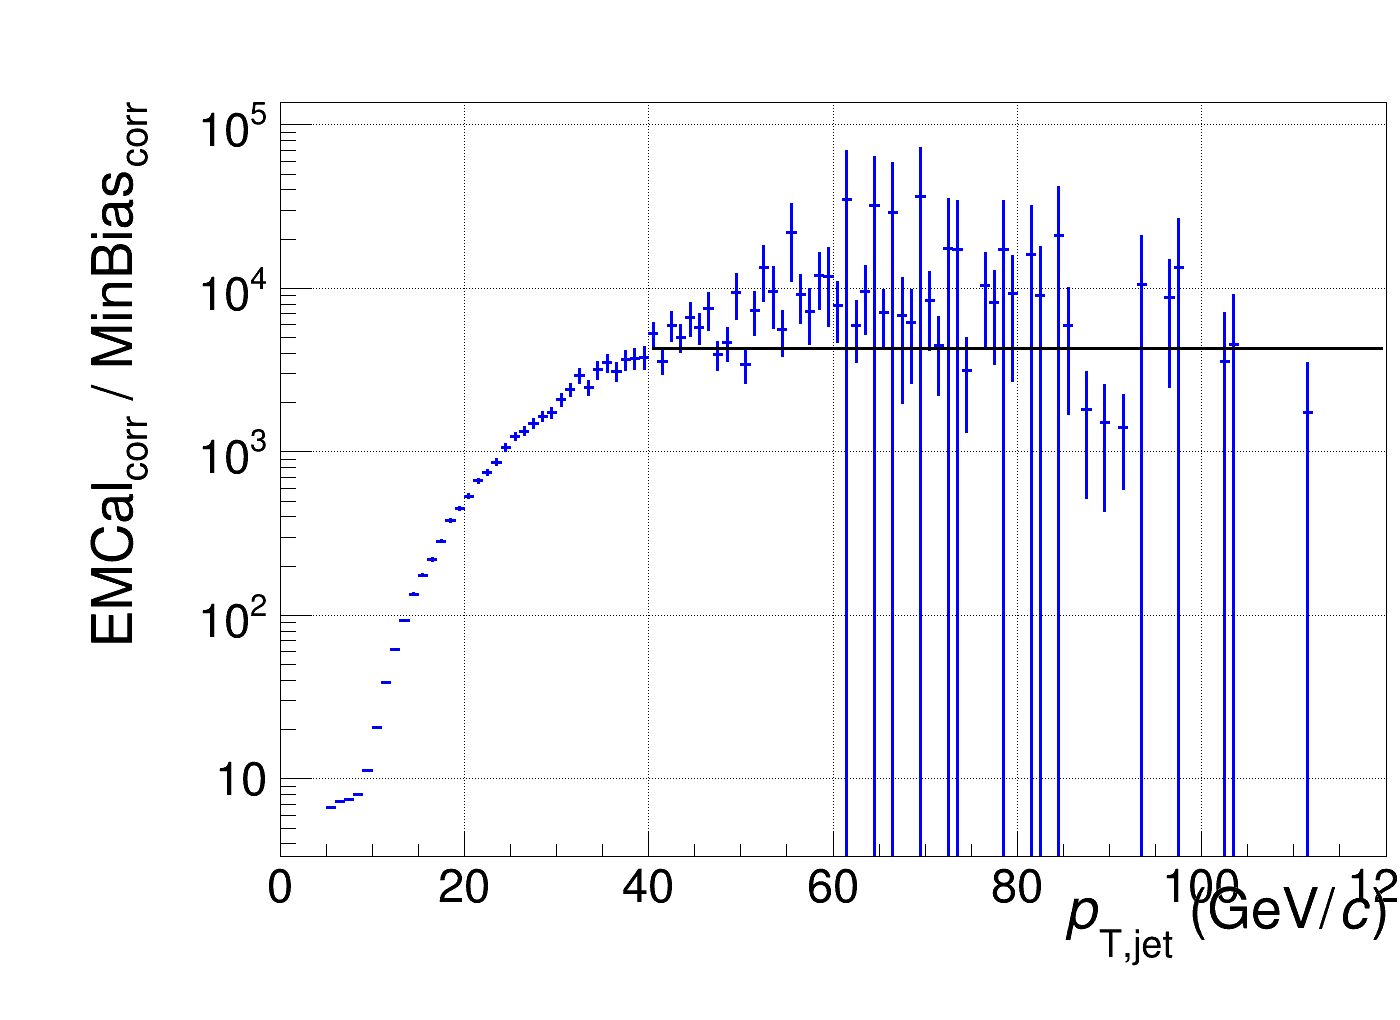
\includegraphics[width=0.5\textwidth]{R04TriggerYields}}
\end{array}$
\caption[EMCal triggered data correction factors for R=0.2, R=0.3, and R=0.4 jets.]{\label{fig:EMCalDownScale}EMCal triggered data correction factors for R=0.2, R=0.3, and R=0.4 jets.}
\end{figure*}
 

\section{Particle Level Corrections}

The reconstructed jet $p_{T}$ is impacted by a number of detector effects:

\begin{itemize}
\item Tracking inefficiencies from the TPC and ITS.
\item Missing jet energy components from long-lived particles, such as the $K^{0}_{L}$ and neutron, that are cut by the EMCal timing requirement.
\item TPC track $p_{T}$ and EMCal cluster energy resolutions.
\item Hadronic corrections to the EMCal cluster spectrum.
\item Material loss in the detectors.
\end{itemize}

\noindent
The magnitude of any one of these inefficiencies may be small but together they can contribute to large discrepancies.  `Bin-by-bin' corrections are a method to correct the uncorrected jet spectra to get a true jet spectrum.  This is then compared with theoretical calculations or other experimental results.

In order to correct the jet spectrum, it is necessary to generate a response matrix that simulates the effects described above.  In order to generate the response matrix, a PYTHIA generated event is propagated through a GEANT based simulation of the ALICE detector.  Each LHC period has a unique simulation produced for it to account for changes in the detector performance.  The differences in the simulations take into account all the hot and dead sectors for the subdetectors, along with their calibrated performance during that specified period.  The bin-by-bin corrections used in this analysis were taken from the PYTHIA simulations produced by ALICE with particles propagated through the detector using GEANT.

\subsubsection{Response Matrix}
The output from the PYTHIA portion of the simulation contains all the final state hadrons, regardless of whether or not they would be detected in the experiment.  This is known as the particle-level.  The particle-level jets are constructed from the PYTHIA final state hadrons.  After the particle-level jet passes through the simulation of ALICE the detector-level jets with the detector effects are obtained.
The response matrix is constructed by geometrically matching particle-level jets to detector-level.  The particle-level jet centroid ($\phi_{part}$,$\eta_{part}$) is matched to the detector-level jet centroid ($\phi_{det}$,$\eta_{det}$) via a constraint on the displaced distance between the two jet centroids.  This distance was constrained to: $\Delta  R = \sqrt{(\phi_{part} - \phi_{det})^{2} + (\eta_{part} - \eta_{det})^{2}} \leq 0.25 \; $.  The response matrix is constructed by averaging over the simulated jets.

\begin{figure}[h]
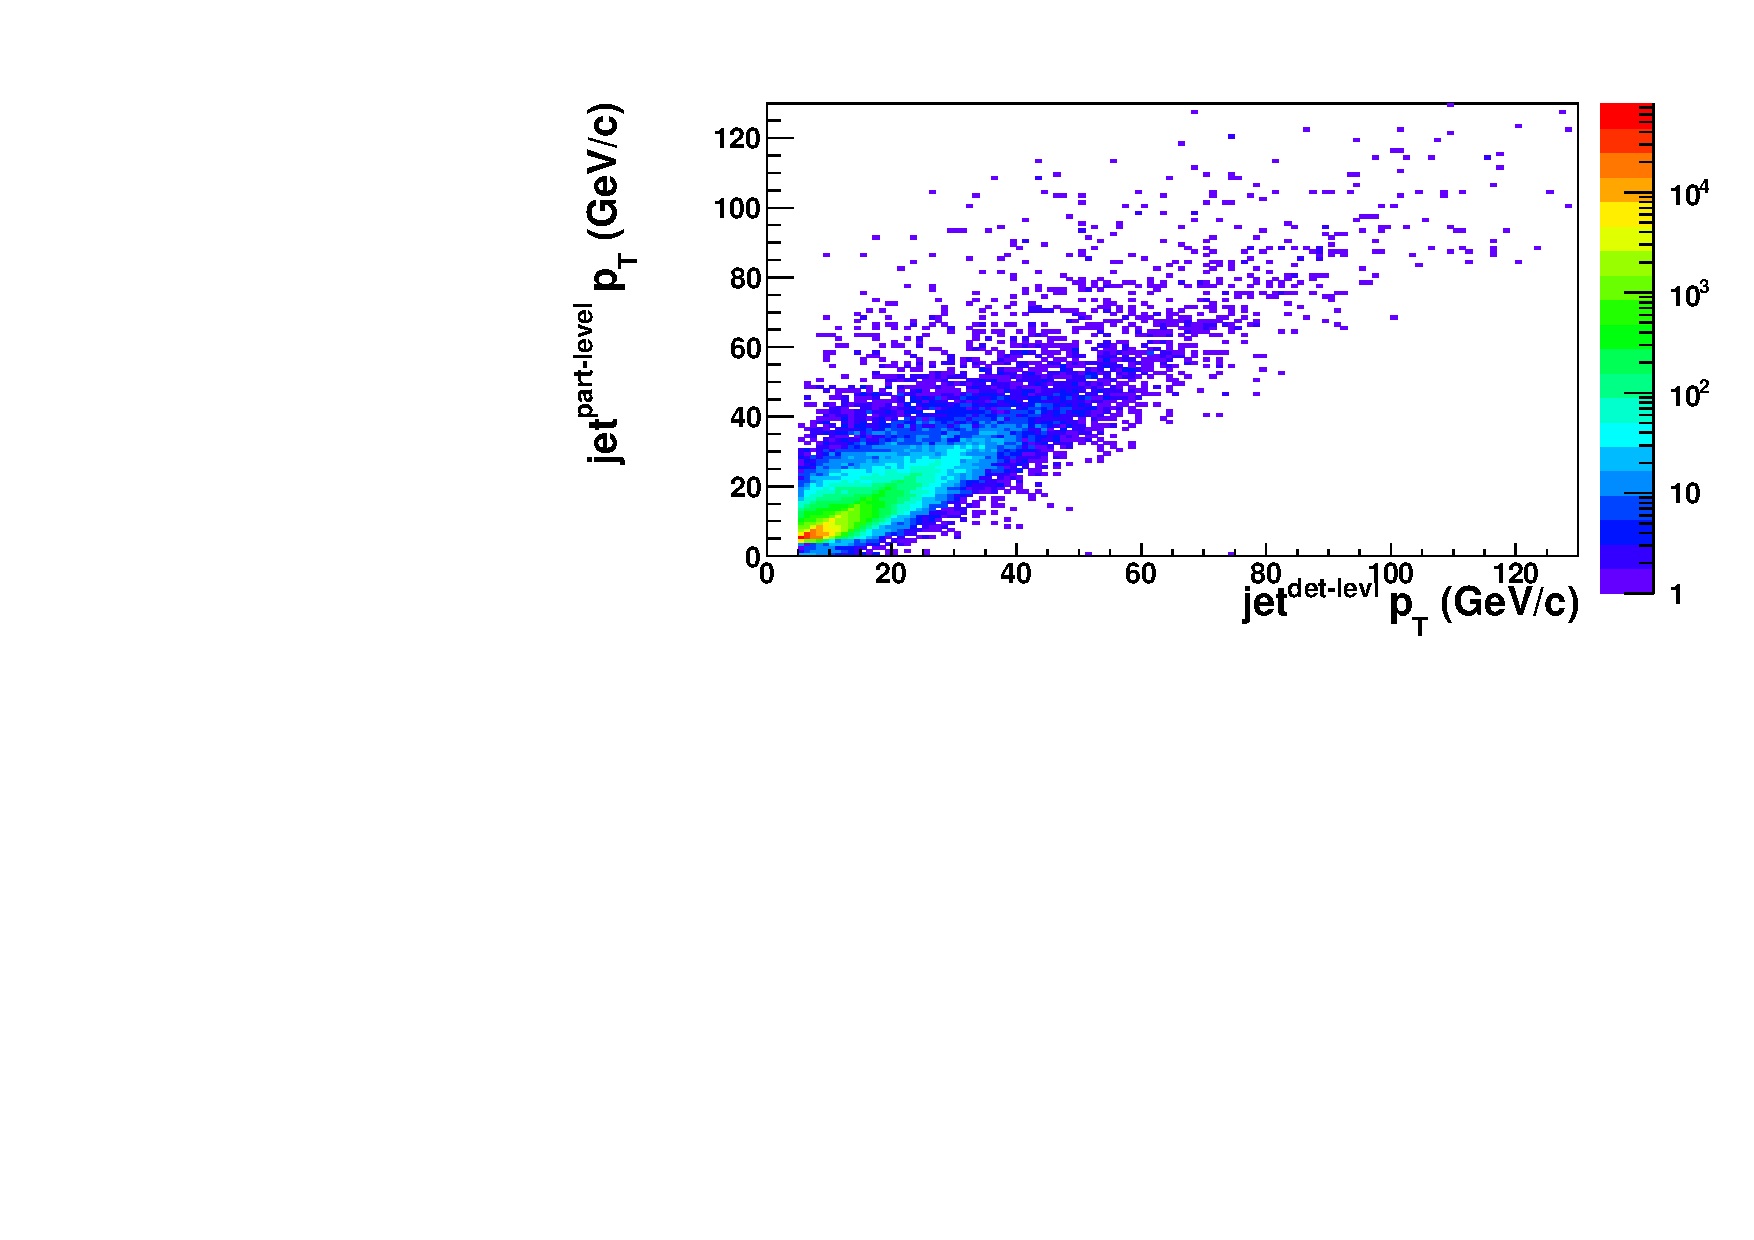
\includegraphics[width=\linewidth]{RMRR}
\centering
\caption{Response Matrix for R = 0.2 jets.}
\label{fig:response}
\end{figure}

Figure \ref{fig:response} shows the response matrix for R = 0.2 jets.  The y-axis shows the jet $p_{T}$ at the particle-level from PYTHIA and the x-axis shows the jet $p_{T}$ after it has been propagated throught the GEANT simulation of ALICE.  The response matrix shows an approximately linear relationship below 50 GeV on both axis and show that above $\sim$100 GeV the matrix lacks statistics.  The jet finder was configured for a minimum jet energy of 100 MeV and no minimum energy requirement at the particle-level.  The detector-level jet finders were configured in the same manner as they were for the uncorrected jet spectra measurement.

\subsubsection{Corrections to particle-level}

Corrections were performed using the \verb+RooUnfold+\cite{Adye:2011gm} software package.  RooUnfold can perform corrections using the bin-by-bin method.  It can also perform unfolding using either the Bayesian or singular value decomposition.  Particle-level corrections were initially attempted using either using either Bayesian or Singular Value Decomposition unfolding but both were unstable due to low statistics. Corrections were applied using the bin-by-bin\cite{Cowan:2002in} algorithm. 

\begin{equation}
C_{MC} \big( p_{T}^{low} : p_{T}^{high} \big) =  \frac{  \int^{p_{T}^{high}}_{p_{T}^{low}} dp_{T} \; \frac{dF^{uncorr}_{meas}}{dp_{T}} \times \frac{d^{2}N^{particle}_{MC}/d\eta \, dp_{T}}{d^{2}N^{detector}_{MC}/d\eta \, dp_{T}}  } { \int^{p_{T}^{high}}_{p_{T}^{low}} dp_{T} \; \frac{dF^{uncorr}_{meas}}{dp_{T}} }
\label{eq:binbybin}
\end{equation}

\noindent
where $d^{2}N^{particle}_{MC}/dp_{T} \, d\eta$ is the PYTHIA particle-level inclusive jet spectra, $d^{2}N^{detector}_{MC}/dp_{T} \, d\eta$ is the detector-level inclusive jet spectra, $dF^{uncorr}_{meas} / dp_{T}$ is a weight function which minimizes the dependence on the two simulation spectra shapes, and finally $p_{T}^{low}$ and $p_{T}^{high}$ are the lower and upper bin limits.  Due to the limited statistics derived from the availabe Monte Carlo simulations, the Bin-by-Bin corrections were stable for a jet momentum range of: $p_{T,jet} \, \, \epsilon \;$ [20 GeV, 120 GeV] for both the uncorrected Min Bias and EMCal triggered data sets.  

\subsubsection{Corrected Jet Spectra}


At low-$p_{T}$ it was observed that the Monte Carlo corrections increased the yield of the spectra while at high-$p_{T} \geq \,$ 40 GeV the yield was decreased for all jet radii in this analysis.  Once the bin-by-bin corrections were performed for the fine binned spectra the output along with the bin-by-bin correction factors were obtained between 10 GeV and 120 GeV.  These corrected spectra are shown in Figures \ref{fig:JetSpecCorrR02}, \ref{fig:JetSpecCorrR03}, and \ref{fig:JetSpecCorrR04}.

\afterpage{%

\begin{figure}
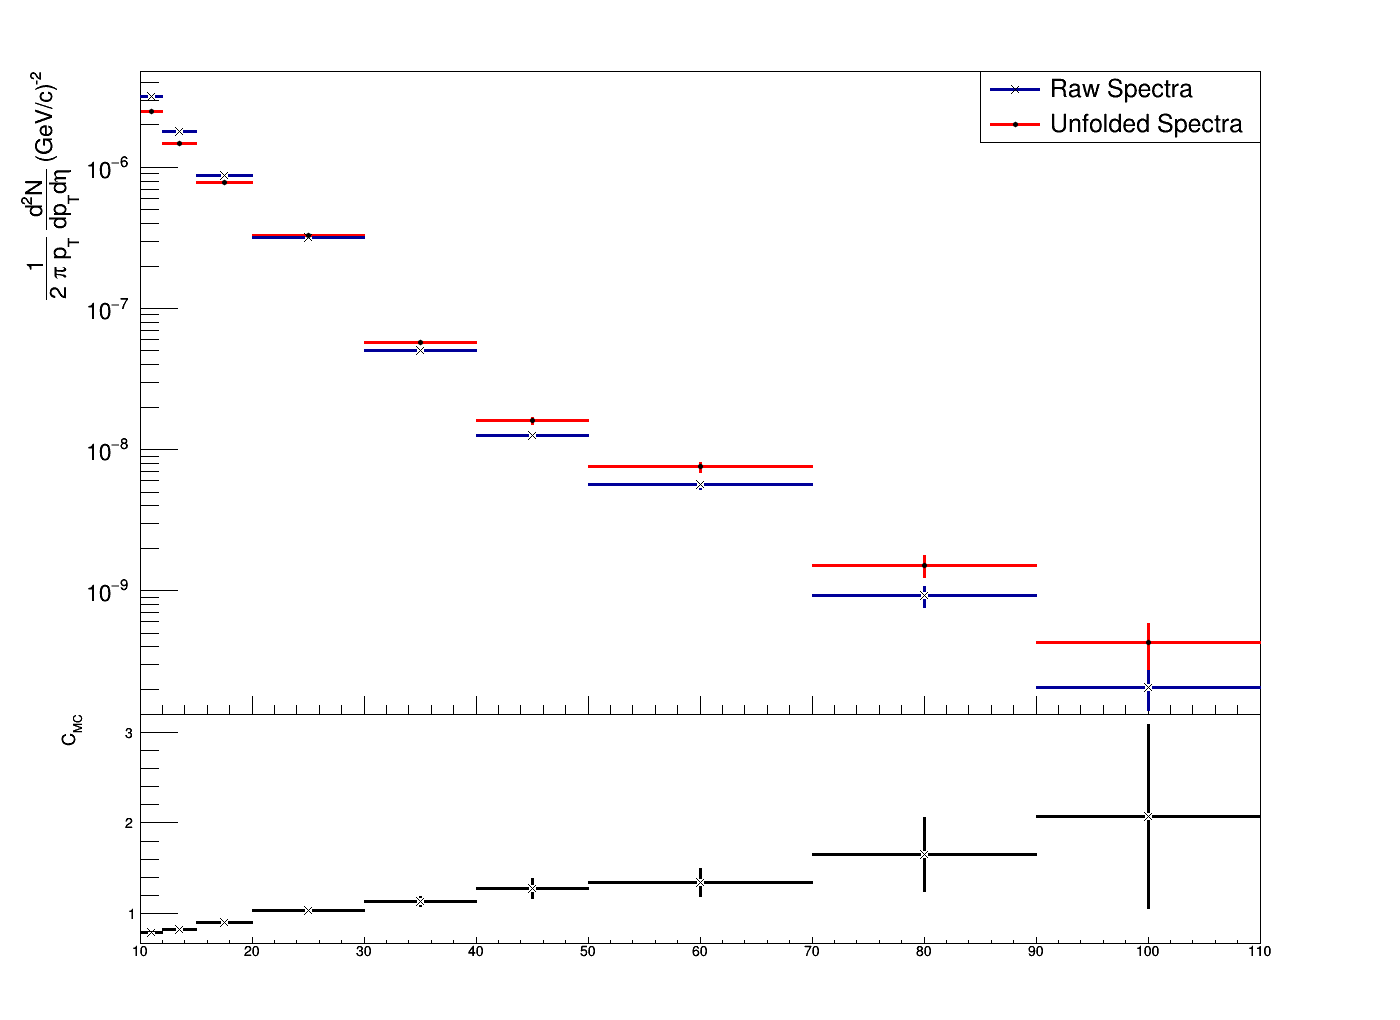
\includegraphics[width=\linewidth]{UnfoldedR02MinBias}
\centering
\caption{R = 0.2 bin-by-bin corrected Min Bias jet spectra.}
\label{fig:JetSpecCorrR02}
\end{figure}

\begin{figure}
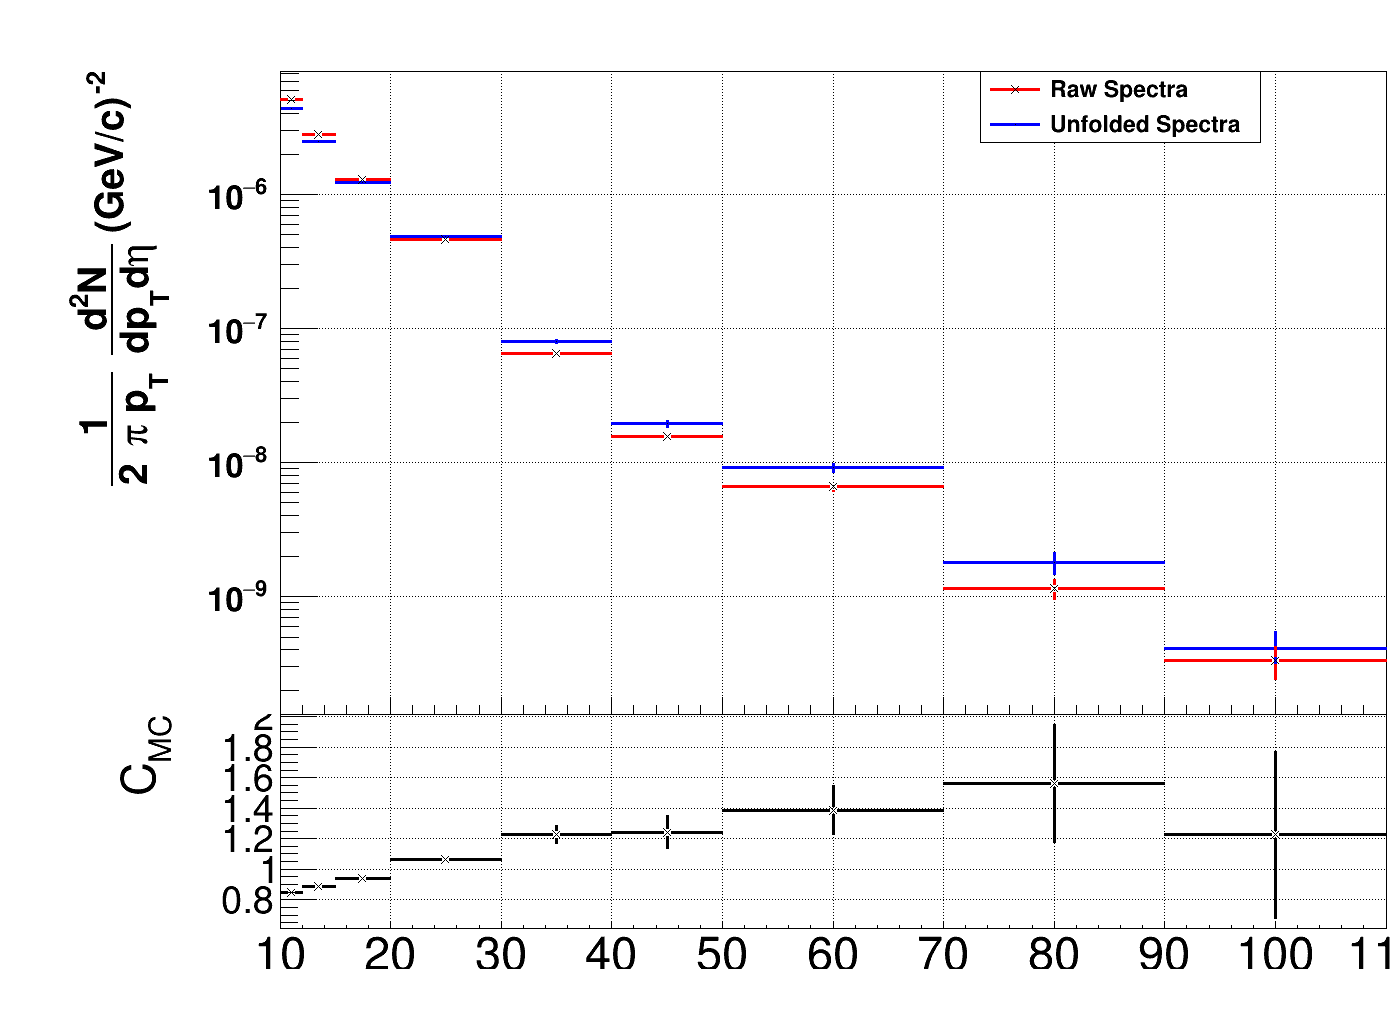
\includegraphics[width=\linewidth]{UnfoldedR03MinBias}
\centering
\caption{R = 0.3 bin-by-bin corrected Min Bias jet spectra.}
\label{fig:JetSpecCorrR03}
\end{figure}

\begin{figure}
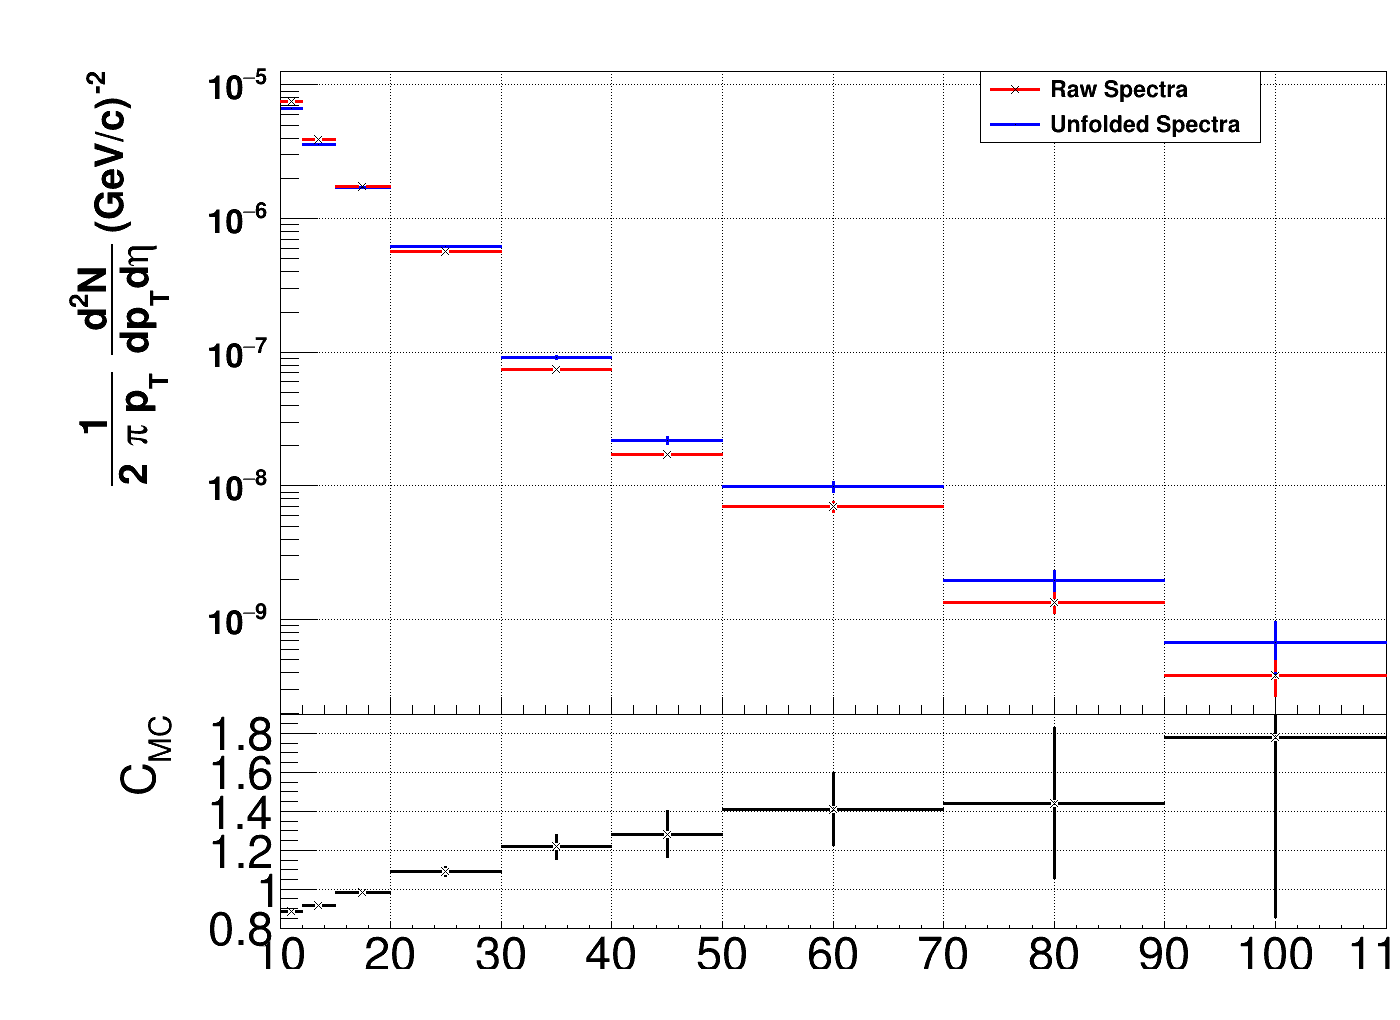
\includegraphics[width=\linewidth]{UnfoldedR04MinBias}
\centering
\caption{R = 0.4 bin-by-bin corrected Min Bias jet spectra.}
\label{fig:JetSpecCorrR04}
\end{figure}

\clearpage
}



\subsubsection{Corrected EMCal Triggered Spectra}
The bin-by-bin correction was repeated again for the EMCal triggered jet spectra.  The response matrix from the Min Bias sample was used for the bin-by-bin correction of the triggered data.  The detector-level and particle-level jets were configured in the same manner as above and the output from the corrected triggered spectra are reported over the same kinematic range as the Min Bias spectra, as seen in Figures \ref{fig:JetSpecCorrEMCR02}, \ref{fig:JetSpecCorrEMCR03}, and \ref{fig:JetSpecCorrEMCR04}.


\afterpage{%

\begin{figure}
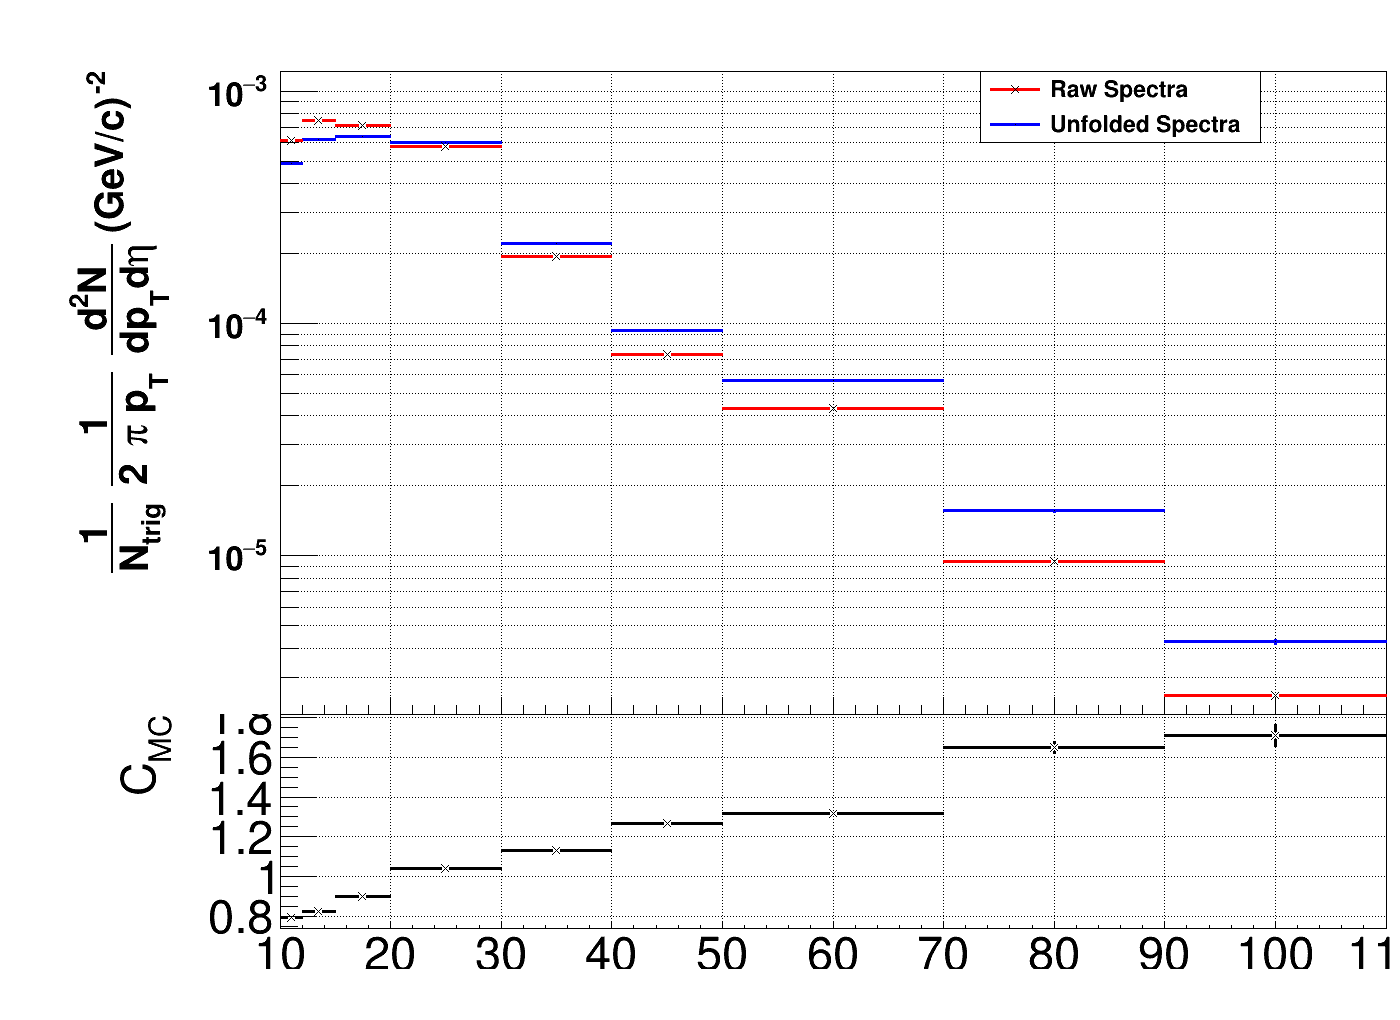
\includegraphics[width=\linewidth]{UnfoldedR02EGAtrigger}
\centering
\caption{R = 0.2 bin-by-bin corrected EMCal triggered jet spectra.}
\label{fig:JetSpecCorrEMCR02}
\end{figure}

\begin{figure}
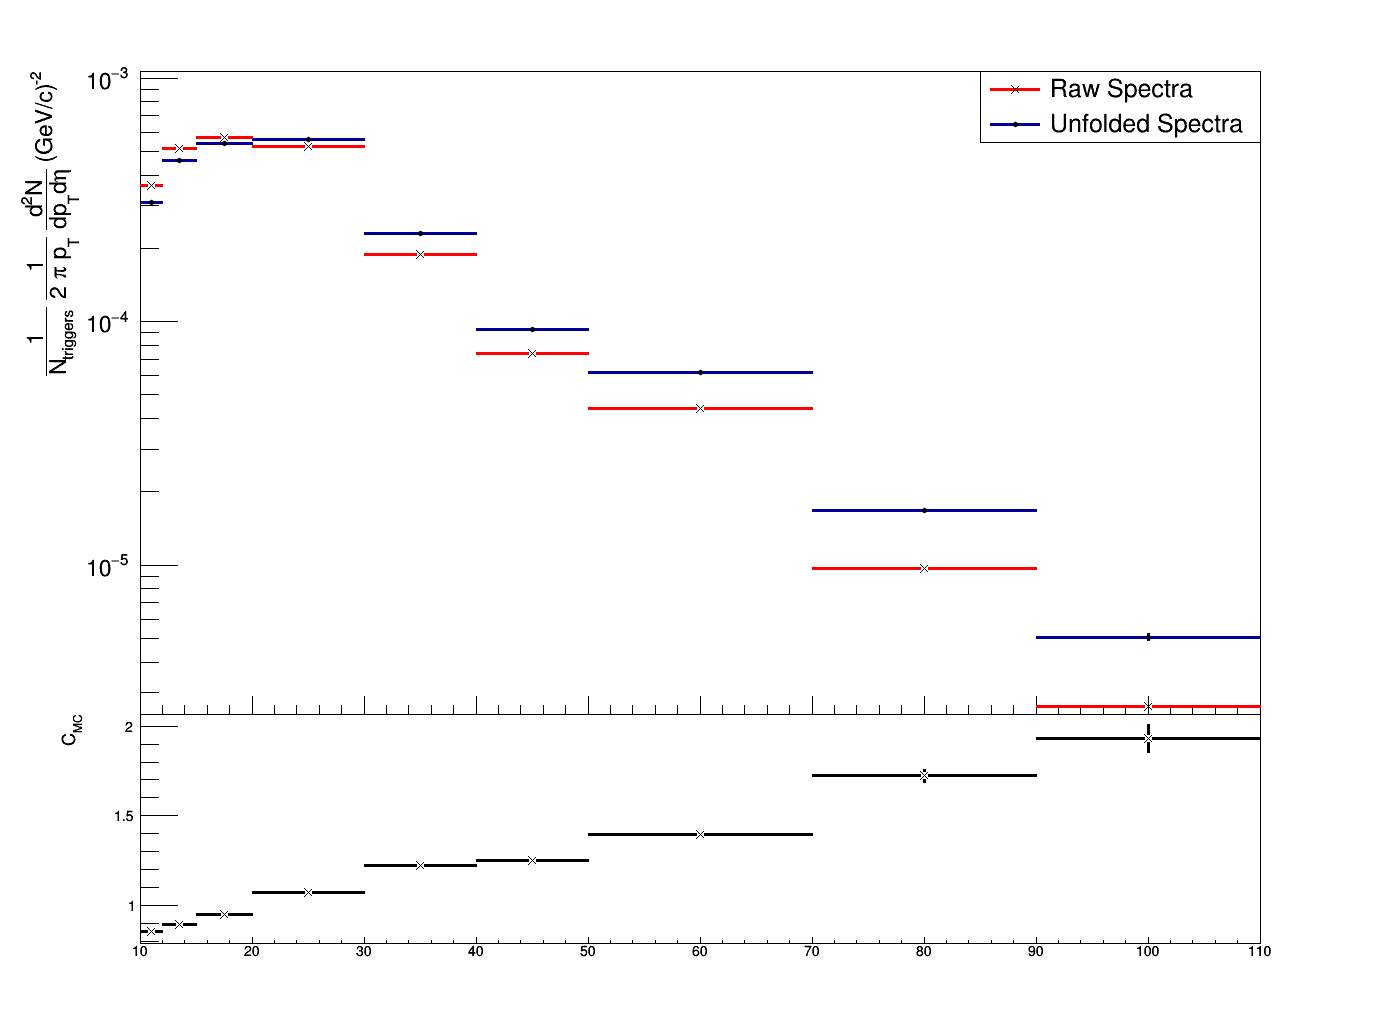
\includegraphics[width=\linewidth]{UnfoldedR03EGAtrigger}
\centering
\caption{R = 0.3 bin-by-bin corrected EMCal triggered jet spectra.}
\label{fig:JetSpecCorrEMCR03}
\end{figure}

\begin{figure}
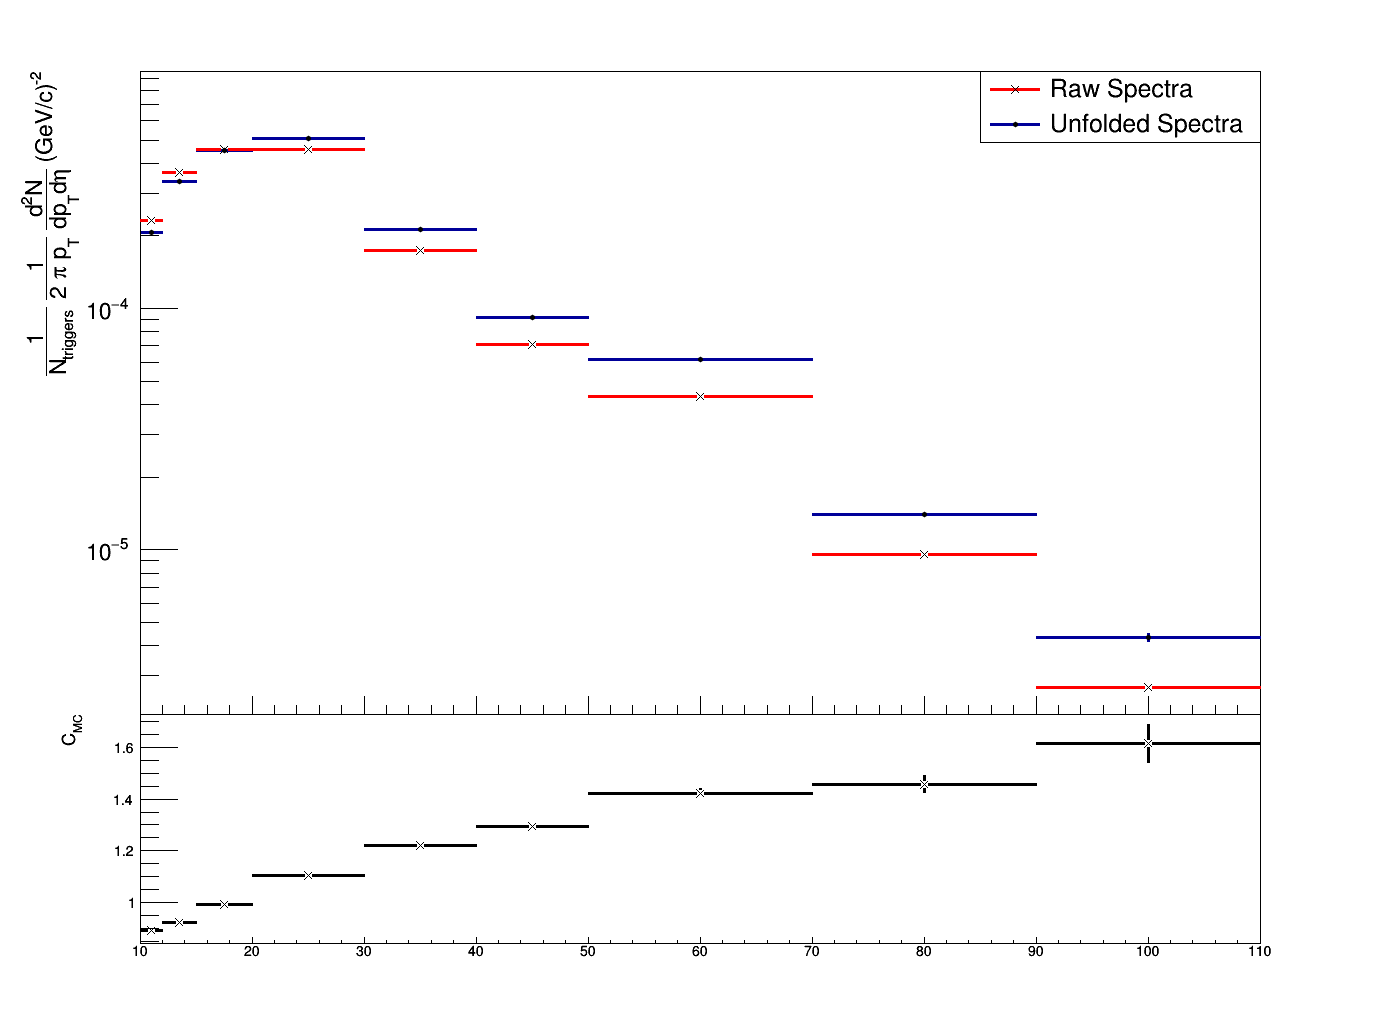
\includegraphics[width=\linewidth]{UnfoldedR04EGAtrigger}
\centering
\caption{R = 0.4 bin-by-bin corrected EMCAL triggered jet spectra.}
\label{fig:JetSpecCorrEMCR04}
\end{figure}

\clearpage
}

Due to the limitations of the response matrix, the bin-by-bin corrections of the EMCal triggered data were used to 120 GeV.  Again, it should be noted that the bumps in the EMCal jet spectra is due to the firing threshold of the trigger.

\section{Jet Reconstruction and Matching Correction}
In order to quantify the inefficiencies due to bin-by-bin corrections and jet reconstructing, we quantify the jet reconstruction efficiency, $\epsilon_{reco} (p_{T, jet})$, and the jet matching efficiency, $\epsilon_{match} (p_{T, jet})$.


\begin{equation}
 \epsilon_{reco} (p_{T, jet}) = \frac{N_{reco}(p_{T, jet}) }{N_{Truth} (p_{T, jet})}
\label{eq:jetrecoeff}
\end{equation}

\begin{equation}
 \epsilon_{match} (p_{T, jet}) = \frac{N_{match}(p_{T, jet}) }{N_{Truth}(p_{T, jet})}
\label{eq:jetmatchoeff}
\end{equation}


\noindent 
where $N_{reco} (p_{T, jet})$ is the reconstructed jet yield at the detector-level per $p_{T}$ bin, $N_{match}(p_{T, jet})$ is the reconstructed jet at the detector-level that was matched to a particle-level jet per $p_{T}$ bin, and $N_{truth} (p_{T, jet})$ is the particle-level jet yield from the PYTHIA embedded event per $p_{T}$ bin.  

The $N_{truth} (p_{T, jet})$ were obtained by running FASTJET on PYTHIA events with no constituent $p_{T}$ cut, while $N_{match}(p_{T, jet})$ and $N_{reco} (p_{T, jet})$ had the same kinematic cuts as the data analysis mentioned earlier in this chapter.  The particle-level jets contained no geometric acceptance cut in order to account for jets that may have been reconstructed at the detector-level, but had no match to a particle-level jet because part of the particle-level jet was outside the EMCal acceptance.  The spectra were corrected by the efficiencies after the bin-by-bin corrections were performed.  The correction factors are shown in Figures \ref{fig:JetMatcheff} and \ref{fig:JetRecoeff}.

\afterpage{%
\begin{figure*}
$\begin{array}{rl}
    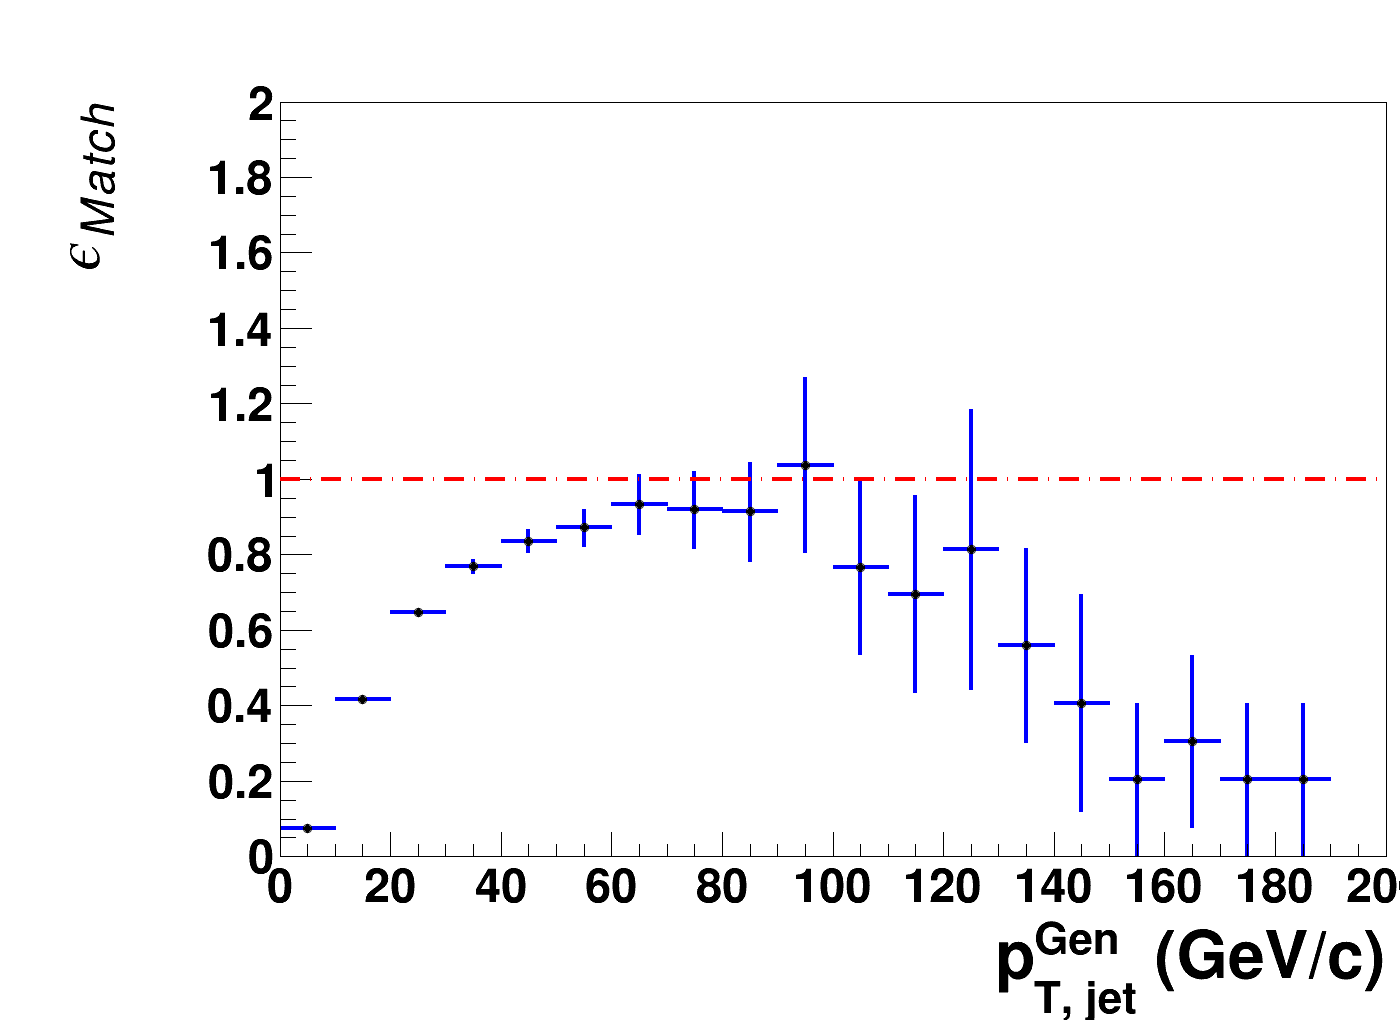
\includegraphics[width=0.5\textwidth]{Ematch_R02} &
    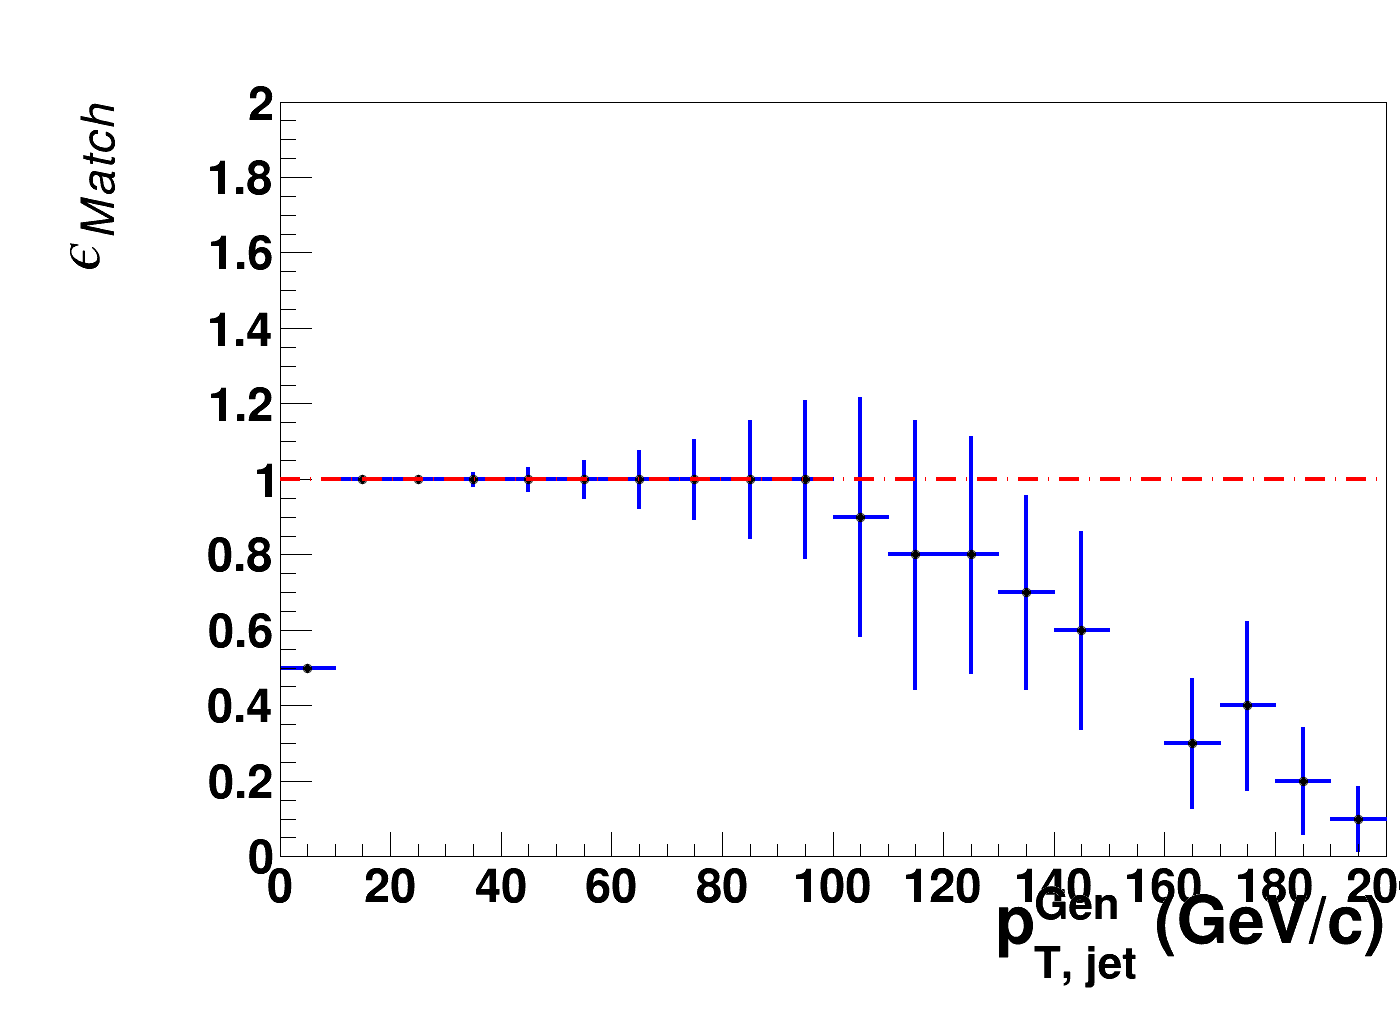
\includegraphics[width=0.5\textwidth]{Ematch_R03}\\
    \multicolumn{2}{c}{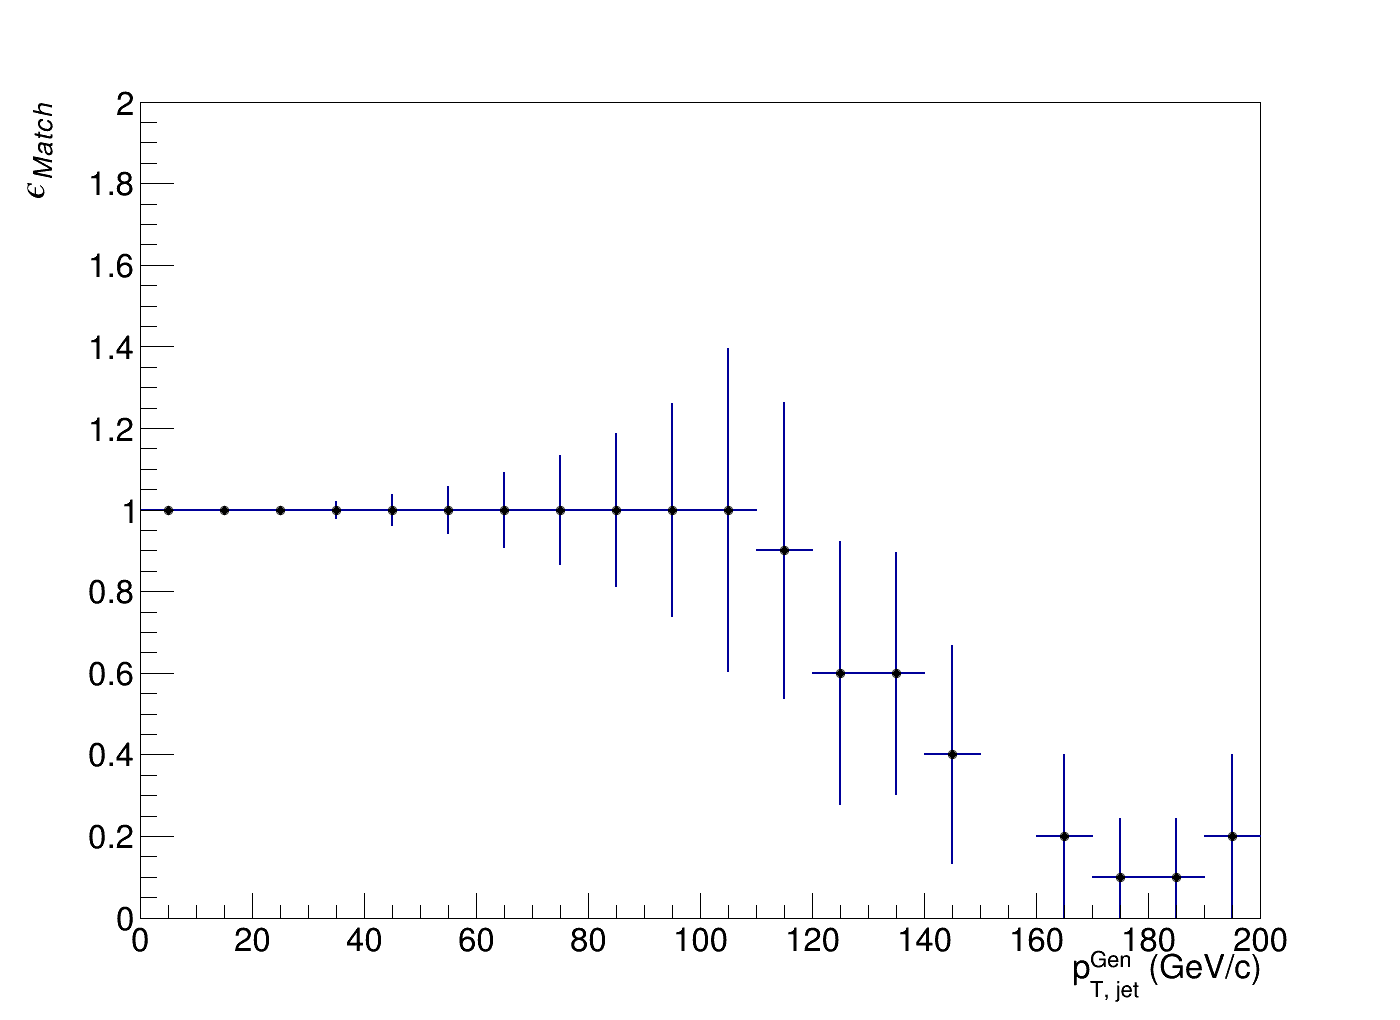
\includegraphics[width=0.5\textwidth]{Ematch_R04}}
\end{array}$
\caption[Jet reconstruction efficiency for jets between R = 0.2 and R = 0.4. ]{\label{fig:JetMatcheff}Jet matching efficiency for jets between R = 0.2 (top left), R = 0.3 (top right), and R = 0.4 (bottom).}
\end{figure*}

\begin{figure*}
$\begin{array}{rl}
    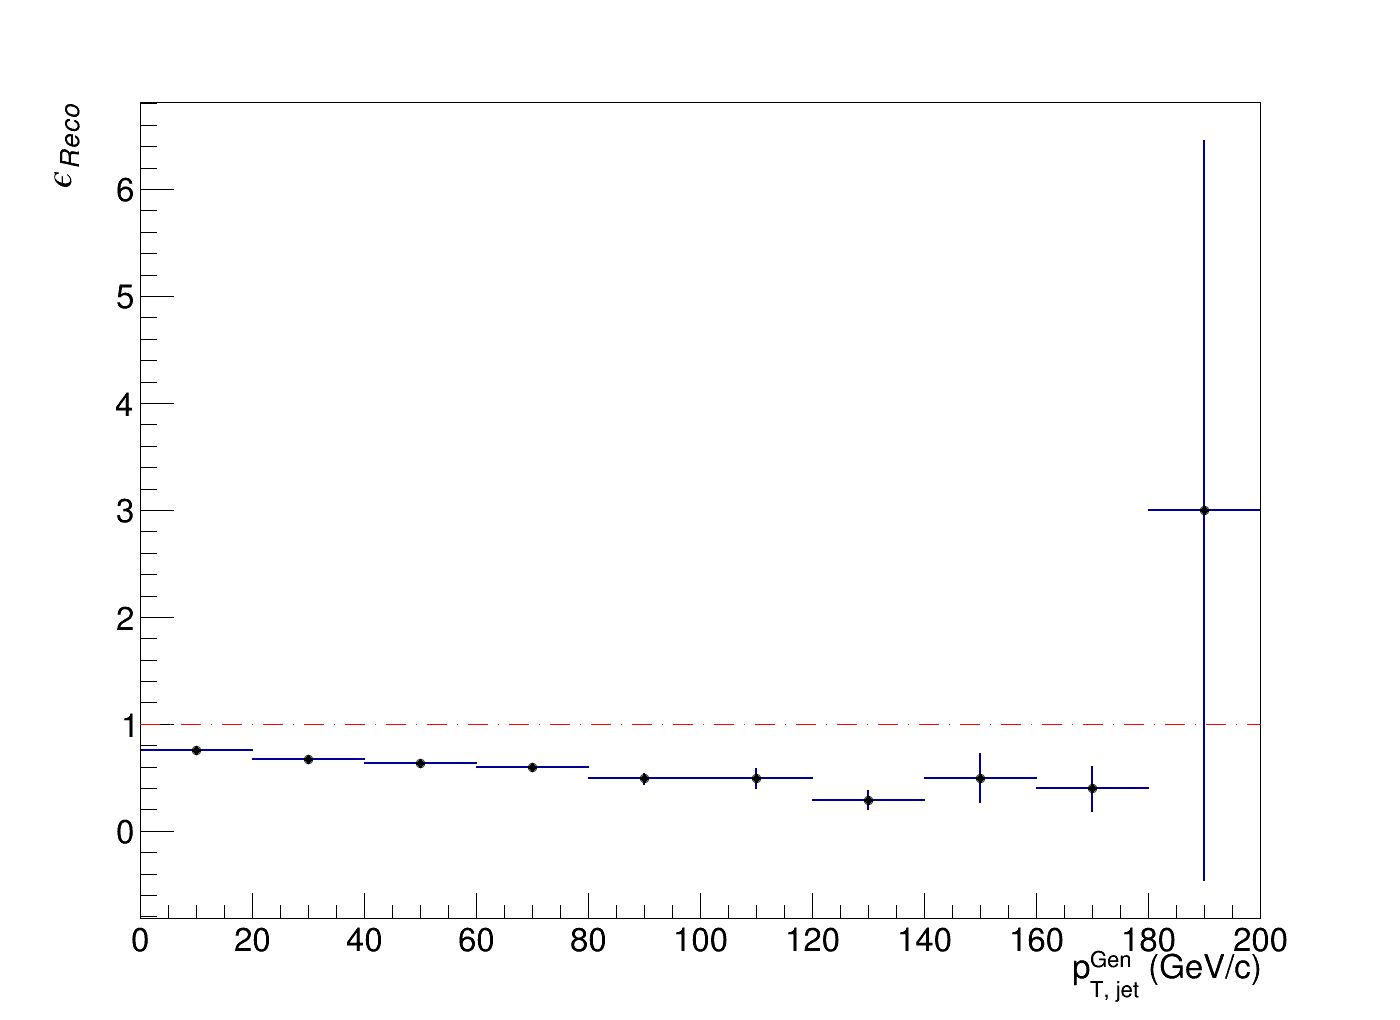
\includegraphics[width=0.5\textwidth]{Ereco_R02} &
    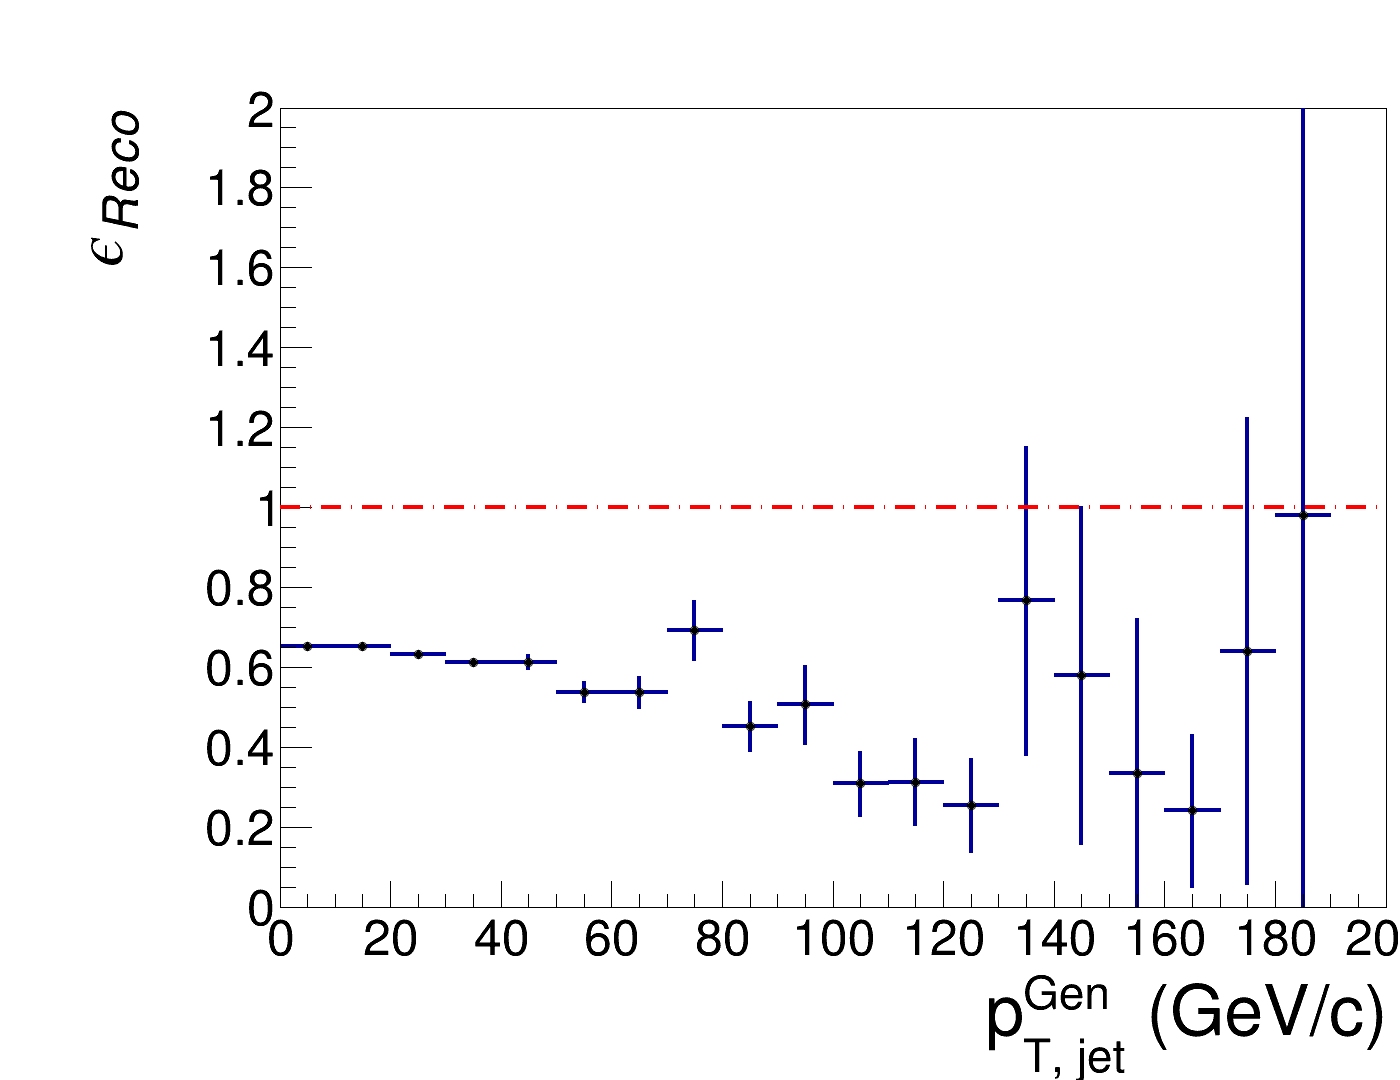
\includegraphics[width=0.5\textwidth]{Ereco_R03}\\
    \multicolumn{2}{c}{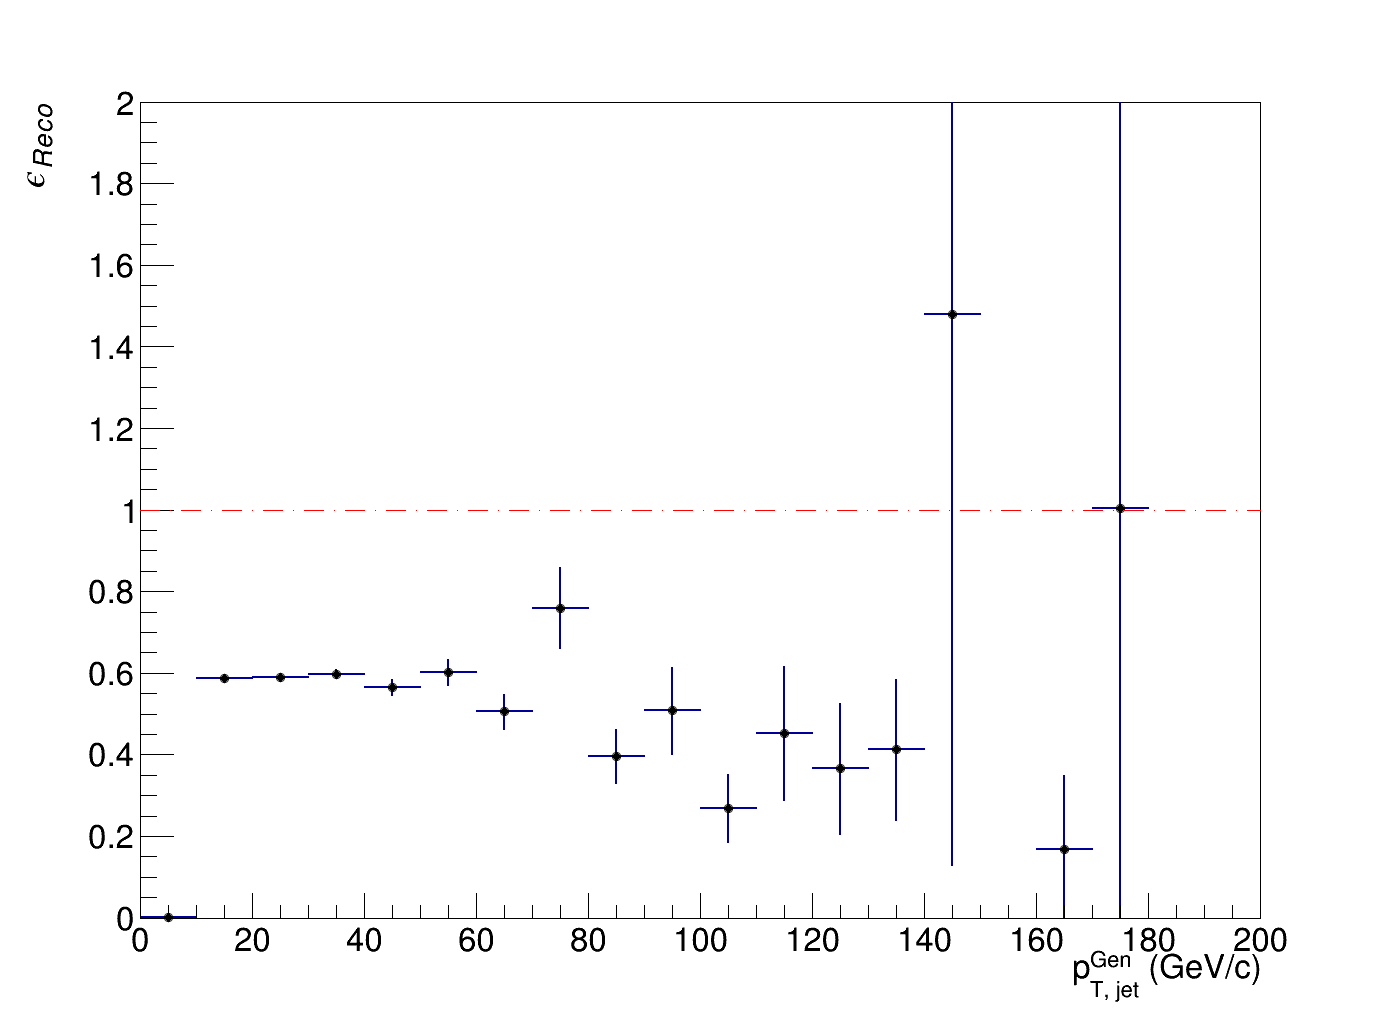
\includegraphics[width=0.5\textwidth]{Ereco_R04}}
\end{array}$
\caption[Jet reconstruction efficiency for jets between R = 0.2 and R = 0.4.]{\label{fig:JetRecoeff}Jet reconstruction efficiency for jets between R = 0.2 (top left), R = 0.3 (top right), and R = 0.4 (bottom)}
\end{figure*}

\clearpage
}

\section{Systematic Uncertainties}

The systematic uncertainties may be broken into two categories: uncertainties in the jet energy scale (JES) which shift the momentum spectra along the momentum axis, and uncertainties in the jet yield, which shift the spectra along the spectra/cross-section axis.  The total systematic uncertainty on the jet cross-section is obtained by adding the JES and yield uncertainties together in quadrature.  The systematic and statistical uncertainties presented in this analysis will be reported as uncertainties on the spectra.  

In general the systematic uncertainties were obtained by using small variations to the parameters used in the analysis..  A feature in some of the following uncertainties is the wide statistical fluctuations seen at the highest jet $p_{T}$ bins.  A small change in a input parameter can cause a relatively large flow into and out of a high granularity bin, which does not represent a systematic uncertainty.  In order to obtain the systematic uncertainty at the highest jet $p_{T}$ bins it was necessary to extrapolate the uncertainty from the low $p_{T}$ range.  Some systematic uncertainties were assigned conservative values due to high statistical fluctuations in the highest $p_{T}$ bins.  

\subsubsection{Systematic Uncertainty in the Jet Energy Scale}

The following sections present and discuss the uncertainties caused by shifts to the JES. 

\subsubsection{Tracking Efficiency Sensitivity}
Only a fraction of charged tracks generated by the hard scattering of two protons will be detected in the TPC due to its finite track reconstruction efficiency.  Uncertainties in the efficiency of the TPC were studied and found to be 5\% for single track reconstruction\cite{Abelev:2013ala}.  In order to obtain the uncertainty on the JES due to the tracking efficiency, this analysis was repeated while throwing out 5\% of the tracks from each event and remeasuring the jet spectra.  Once this new jet spectrum was generated, it was corrected using the bin-by-bin corrections and the ratio of this new spectra were taken with the original spectra to gauge the uncertainty from the tracking efficiency.


\begin{figure*}[t!]
$\begin{array}{rl}
    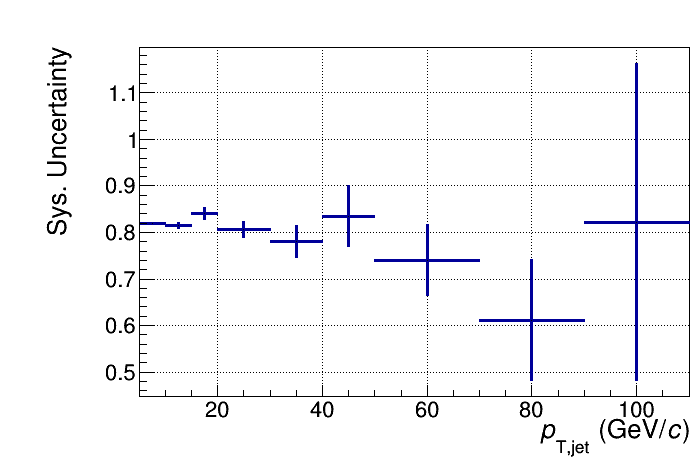
\includegraphics[width=0.40\textwidth]{SysR02_TrkEff} &
    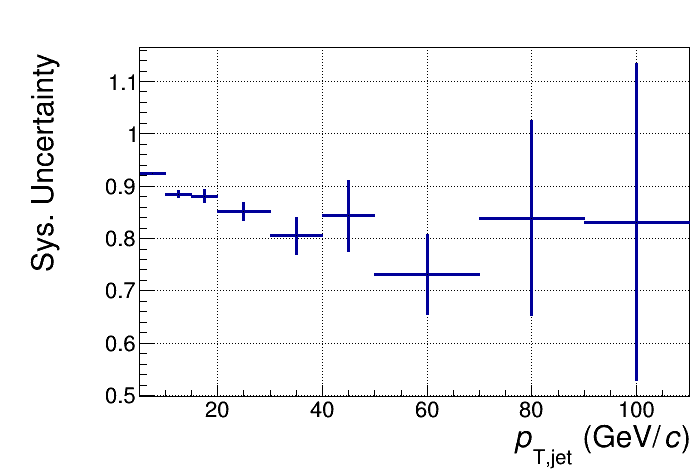
\includegraphics[width=0.40\textwidth]{SysR03_TrkEff}\\
    \multicolumn{2}{c}{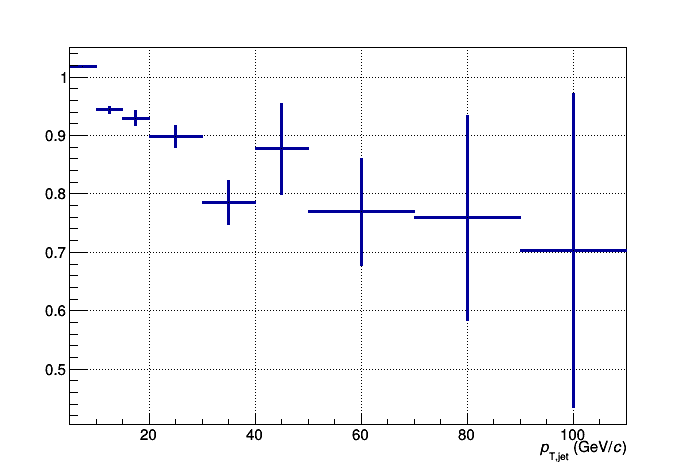
\includegraphics[width=0.40\textwidth]{SysR04_TrkEff}}
\end{array}$
\caption[Systematic due to TPC tracking efficiency.]{\label{fig:trkeff}Systematic uncertainty due to TPC tracking efficiency; R = 0.2 \textit{(top left)}, R = 0.3 \textit{(top right)}, R = 0.4 \textit{(bottom)}.}
\end{figure*}


Figure \ref{fig:trkeff} shows the systematic uncertainties for R = 0.2, R = 0.3, and R = 0.4 jets.  Based on the analysis a 10\% systematic was assigned to R = 0.2 and R = 0.3 jets, while a 15\% systematic uncertainty was given to R = 0.4 jets for this analysis.

\subsubsection{Hadronic Correction}

\begin{figure*}[t!]
$\begin{array}{rl}
    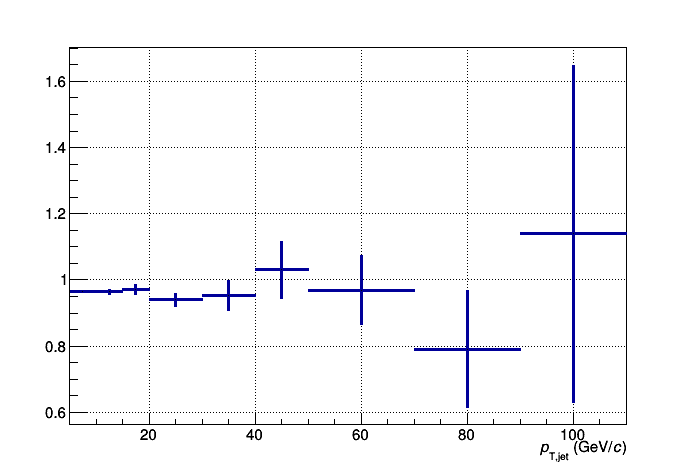
\includegraphics[width=0.40\textwidth]{SysR02_F07} &
    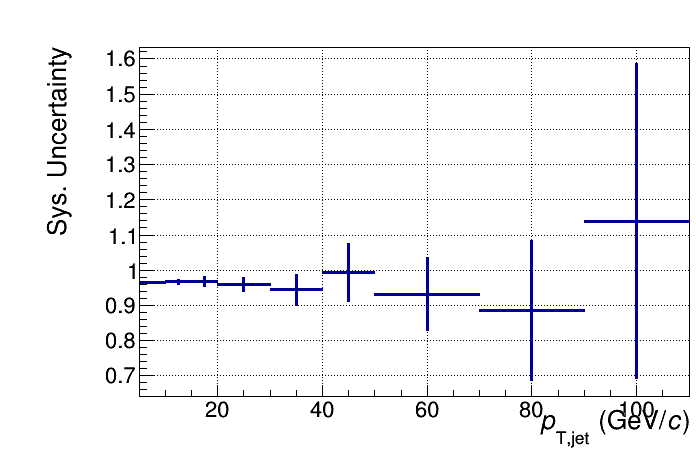
\includegraphics[width=0.40\textwidth]{SysR03_F07}\\
    \multicolumn{2}{c}{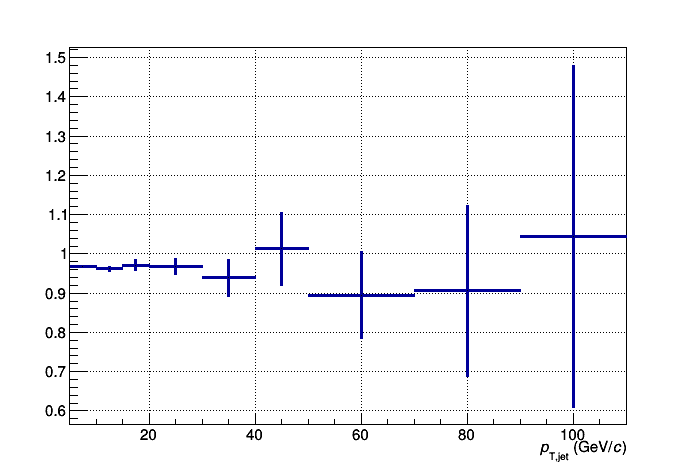
\includegraphics[width=0.40\textwidth]{SysR04_F07}}
\end{array}$
\caption[Systematic due to Hadronic correction.]{\label{fig:hadeff}Systematic uncertainty due to hadronic correction efficiency; R = 0.2 \textit{(top left)}, R = 0.3 \textit{(top right)}, R = 0.4 \textit{(bottom)}.}
\end{figure*}

The uncertainty in the JES due to the hadronic correction applied to EMCal clusters was measured by changing the nominal value of $f_{sub} = 1$ in equation \ref{eq:HadCorr} to 0.7 and the analysis chain is repeated.  Figure \ref{fig:hadeff} shows the ratio of the new spectra with the original, and the uncertainty due to the hadronic correction was around 5\% for all jet radii.

\subsubsection{Sensitivity to EMCal Clusterization Algorithm}
The clusterization algorithm, discussed in Chapter \ref{ch:data}, limits the number of EMCal towers in a cluster to a maximum of nine.  In principle jets should not be sensitive to the clustering algorithm because of jet finder clusters these objects into jet candidates. In practice there is some sensitivity.  In order to test the sensitivity the JES has to the clusterization algorithm, a different algorithm was chosen and a new spectra were generated.  The new algorithm is similar to the original algorithm with the exception that the total size of the cluster is forced to be smaller than nine towers.  Similar to the other systematic uncertainties presented, we see large fluctuations at high-$p_{T}$ due to sparsely filled bins in the histograms.  

\begin{figure*}[t!]
$\begin{array}{rl}
    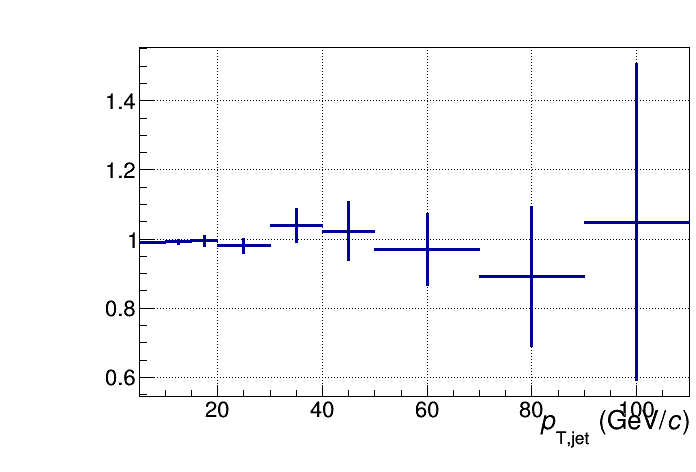
\includegraphics[width=0.40\textwidth]{SysR02_v1Clusterization} &
    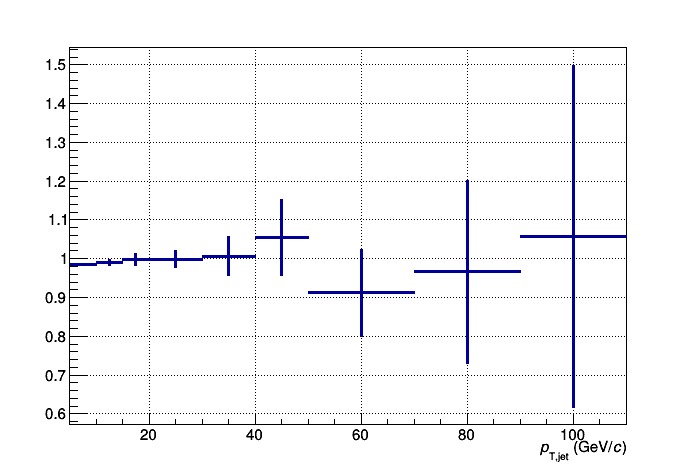
\includegraphics[width=0.40\textwidth]{SysR03_v1Clusterization}\\
    \multicolumn{2}{c}{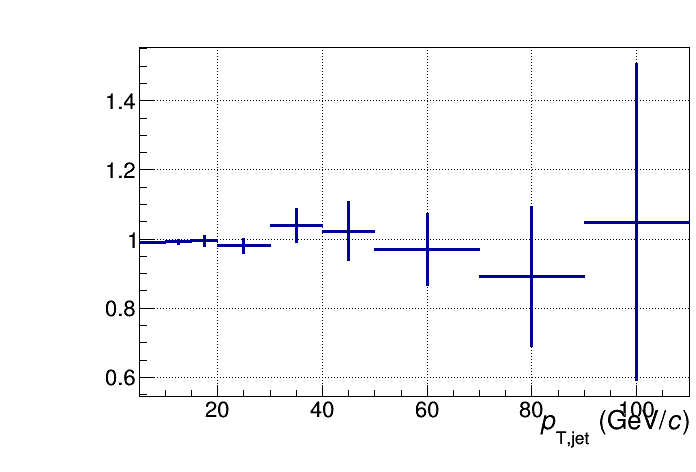
\includegraphics[width=0.40\textwidth]{SysR02_v1Clusterization}}
\end{array}$
\caption[Systematic due to clusterization algorithm.]{\label{fig:cluseff}Systematic uncertainty due to EMCal clusterization algorithm; R = 0.2 \textit{(top left)}, R = 0.3 \textit{(top right)}, R = 0.4 \textit{(bottom)}.}
\end{figure*}

Figure \ref{fig:cluseff} shows the systematic uncertainty due to the clusterization for each of the jet radii.  At low-$p_{T}$ I assigned an uncertainty of between 1\% and 3\% for a given jet radii.  At high-$p_{T}$ I assigned a 5\% for R = 0.2 and 10\% uncertainty for R = 0.3 and R=0.4 jets to account for the statistical fluctuations.

\subsubsection{Systematic Uncertainty on the Jet Yield}

The following sections discuss the systematic uncertainties affecting the jet yield.

\subsubsection{Track $p_{T}$ Resolution}


\begin{figure*}[t!]
$\begin{array}{rl}
    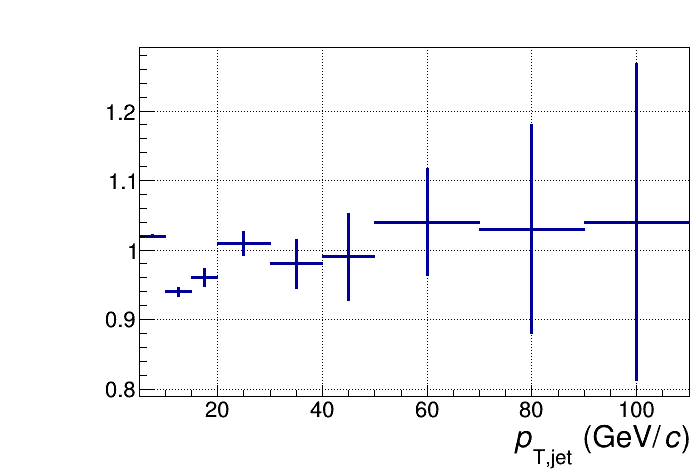
\includegraphics[width=0.40\textwidth]{SysR02_PtReso} &
    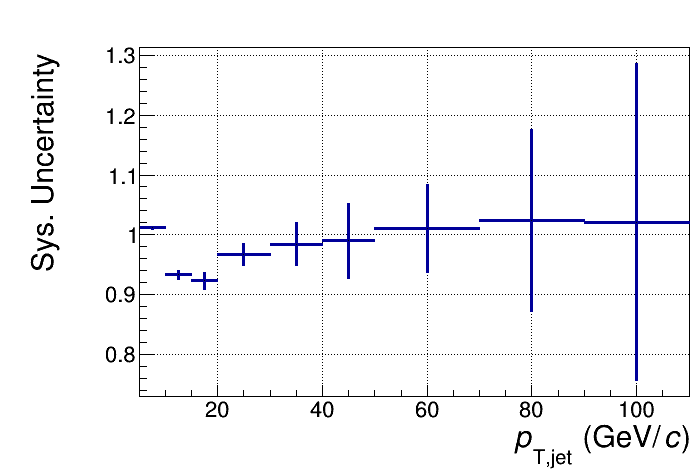
\includegraphics[width=0.40\textwidth]{SysR03_PtReso}\\
    \multicolumn{2}{c}{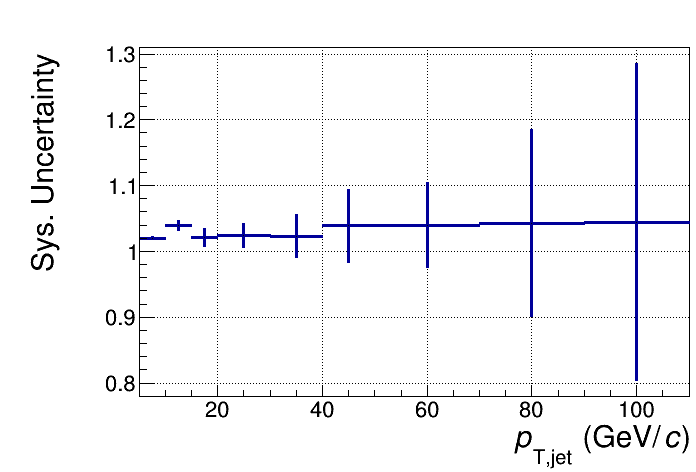
\includegraphics[width=0.40\textwidth]{SysR04_PtReso}}
\end{array}$
\caption[Systematic due to $P_{T}$ resolution.]{\label{fig:pTeff}$P_{T}$ resolution systematic uncertainty; R = 0.2 \textit{(top left)}, R = 0.3 \textit{(top right)}, R = 0.4 \textit{(bottom)}.}
\end{figure*}

\noindent
The momentum resolution of the TPC is estimated using the covariance matrix generated from the Kalman filtering\cite{Fruhwirth:1987fm}.  Figure \ref{fig:trackresolution} shows that for the vast majority of the $p_{T}$ range in this analysis the  momentum resolution is below 3\%.  To estimate the systematic uncertainty due to the $p_{T}$ resolution, tracks are smeared by 3\% in $p_{T}$ and the variation between the new and original spectra are used to estimate the uncertainty.  From the generated plots seen in Figure \ref{fig:pTeff} the uncertainties were below 5\% for all jet radii.

\subsubsection{Cluster Energy Resolution}

\begin{figure*}[t!]
$\begin{array}{rl}
    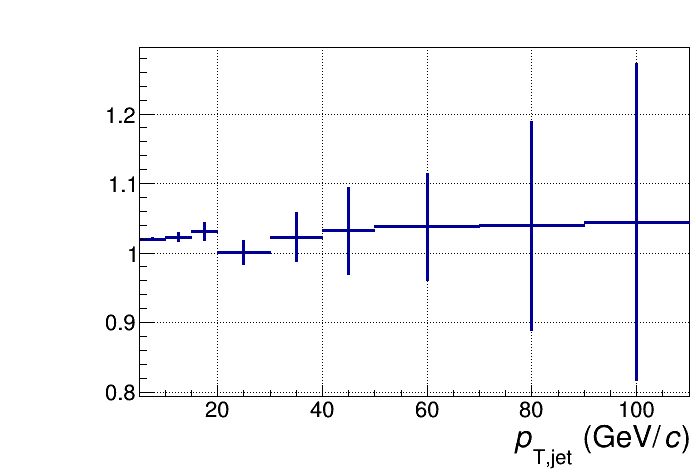
\includegraphics[width=0.40\textwidth]{SysR02_EReso} &
    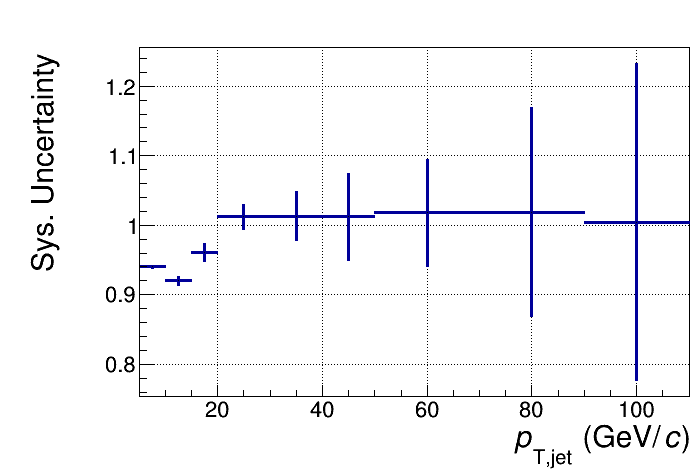
\includegraphics[width=0.40\textwidth]{SysR03_EReso}\\
    \multicolumn{2}{c}{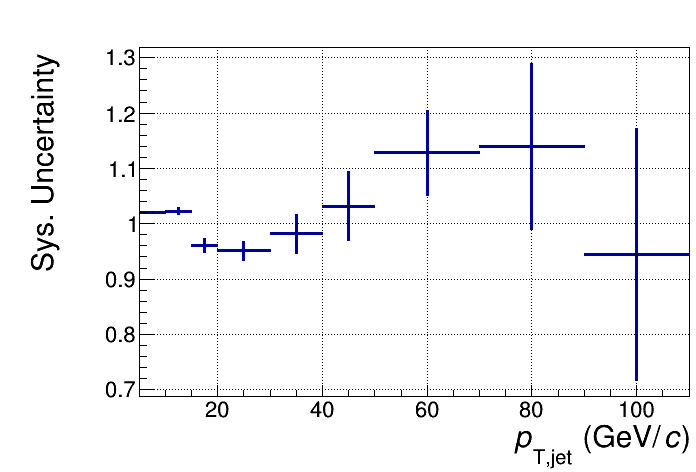
\includegraphics[width=0.40\textwidth]{SysR04_EReso}}
\end{array}$
\caption[Systematic due to energy resolution.]{\label{fig:Eeff}Systematic uncertainty due to the energy resolution; R = 0.2 \textit{(top left)}, R = 0.3 \textit{(top right)}, R = 0.4 \textit{(bottom)}.}
\end{figure*}

Similar to the $p_{T}$ resolution, the uncertainty due to the EMCal energy resolution is done by smearing the energy of the clusters.  The smearing is based on the energy resolution measured from the test beam, and seen in Figure \ref{fig:EMCalres}.  The ratio of the smeared spectra to the original spectra are show in Figure \ref{fig:Eeff}. The uncertainties for the R = 0.2 and R = 0.3 jets are well defined and around 1\% - 2\%.  The large variation with R = 0.4 jet energy resolution is due to large statistical fluctuations and a conservative 5\% uncertainty was assigned to this radii.

\subsubsection{Luminosity Uncertainty}

The luminosity of a hadronic collider, $\mathscr{L}$, is given by the expression,



\begin{equation}
\mathscr{L} = \frac{R}{\sigma}
\label{eq:xlumdef}
\end{equation}

\noindent
where R is the interaction rate and $\sigma$ is the visible cross section.  Due to the fact that we only measure events within a 10 cm window within the primary vertex region of ALICE we must scale the total luminosity to that which is delivered within the experiment.  This scale factor is determined by dividing the total number of Min Bias events to those accepted within the 10 cm window.  $N^{tot}_{MB} / N^{10 cm vertex}_{MB}$ = 1.024, which was obtained from the event QA criteria used in this analysis as discussed in Chapter \ref{ch:data}.
The total cross-section and luminosity along with the uncertainties were determined during a special 8 TeV Van der Meer scan run performed in April of 2012\cite{ALICE-PUBLIC-2017-002}.  The total systematic uncertainty for the Min Bias trigger was obtained by measuring the visible cross-section using the T0 and V0 detectors.  The Min Bias trigger was defined as V0AND which required a hit in both the V0A and V0C.  The cross-section was reported as being a combined average for Min Bias with the V0AND as $\sigma_{V0} = (55.8 \pm 1.2) \, mb$ with a combined systematic uncertainty of 2.19\% on the visible cross section and 2.60\% on the luminosity.  Both this cross-section and its uncertainty were scaled by the 1.024 factor to account for the 10 cm vertex region in ALICE before combining with the spectra to obtain the final cross-sections.


\subsubsection{Total Uncertainty}

A summary of the total systematic uncertainties used in the final analysis is given in Table \ref{table:1}.  Some of the uncertainties, for example the $p_{T}$ resolution, are momentum dependent.  The systematic uncertainties on the yield and JES were added in quadrature.
\newline

\begin{table}[h!]
\centering
\caption{Summary of JES and Yield Uncertainties.}
\begin{tabular}{ |p{5cm}||p{3cm}|p{3cm}|p{3cm}|  }
 \hline
 \multicolumn{4}{|c|}{Systematic Errors} \\
 \hline
 Systematic &R = 0.2 Jets & R = 0.3 Jets& R = 0.4 Jets\\
 \hline
Clusterization (below 40 GeV/\textit{c}) & 1.0\%    &1.0\%&  3.0\%\\
 (above 40 GeV/\textit{c})           &  5.0\%  & 10.0\%   &  10.0\%\\
Hadronic &   5.0\% & 4.0\% & 5.0\%\\
Track Eff (below 40 GeV/\textit{c})&20.0\% & 15.0\% & 15.0\%\\
 (above 40 GeV/\textit{c})            &  25.0\%  & 20.0\%   &  25.0\%\\
Unfolding & 6.0\% & 6.0\%&  6.0\%\\
$p_{T}$ Resolution & 2.0\% & 1.0\% & 4.0\%\\
E Resolution& 2.0\%   &1.0\% & 5.0\%\\
Luminosity & 2.2\%  & 2.2 \% & 2.2\%\\
 \hline
 \hline
Total Sys (low-$p_{T}$) & 8.9\%  & 6.6\% & 10.9\%\\
(high-$p_{T}$) & 10.3\%  & 9.1 \% & 14.5\%\\
\hline
\end{tabular}

\label{table:1}
\end{table}


